
\documentclass[11pt,a4paper]{article}

% =================================================
% PACKAGES
% =================================================
\usepackage[margin=1in]{geometry}
\usepackage{graphicx}
\usepackage{amsmath,amssymb}
\usepackage{booktabs}
\usepackage{caption}
\usepackage{subcaption}
\usepackage{float}
\usepackage{enumitem}
\usepackage{tabularx}
\usepackage{longtable}
\usepackage{threeparttable}
\usepackage{xcolor}
\usepackage[hidelinks]{hyperref}
\usepackage{listings}
\usepackage{setspace}
\usepackage{array}
\usepackage{multirow}

\onehalfspacing

% =================================================
% IMAGE DIRECTORY
% All images are stored in output/figures/images/
% =================================================
\graphicspath{{outputs/figures/}}

\captionsetup{
    font=small,
    labelfont=bf
}

% =================================================
% CODE LISTING SETTINGS
% =================================================
\lstset{
    basicstyle=\ttfamily\small,
    breaklines=true,
    frame=single,
    numbers=left,
    numberstyle=\tiny,
    captionpos=b
}

% =================================================
% TITLE INFORMATION
% =================================================
\title{
    \textbf{Topological and Structural Analysis of the Indian Stock Market}
}

\author{
    Prakhar Chandra\\
    ECS414/614 -- Network Science: Theory and Applications\\
    Under the Guidance of Prof. Kundan Kandhway
}

\date{20 November 2026}

% =================================================
% DOCUMENT
% =================================================
\begin{document}

% =================================================
% TITLE PAGE
% =================================================
\begin{titlepage}
    \centering

    \vspace*{1.5cm}

    {\Large \textbf{NETWORK SCIENCE: THEORY AND APPLICATIONS}}\\[0.5cm]

    {\large ECS414/614}\\[2cm]

    {\huge \textbf{Topological and Structural Analysis of the Indian Stock Market}}\\[2cm]

    {\Large Project Report}\\[1.5cm]

    \textbf{Submitted by}\\[0.3cm]
    {\Large Prakhar Chandra}\\[1cm]

    \textbf{Under the Guidance of}\\[0.3cm]
    {\large Prof. Kundan Kandhway}\\[2cm]

    \vfill

    {\large Academic Term: 2026--27 (I)}\\[0.3cm]
    {\large Submission Date: 20 November 2026}

\end{titlepage}

\tableofcontents
\newpage

% =================================================
\section{Executive Summary}
% =================================================

The Indian stock market consists of companies operating across
different sectors, including banking, financial services,
information technology, healthcare, energy, manufacturing and
consumer goods. The stock prices of these companies may be
connected through common economic conditions, industry-specific
factors and market-wide movements.

This project applies Network Science techniques to examine the
relationships among companies listed in the Indian stock market.
A correlation-based network is constructed using the daily
logarithmic returns of companies belonging to the Nifty 200 index.

The initial dataset contains 200 companies. Historical adjusted
closing prices were collected for the period from 1 November 2023
to 31 October 2026. Following data-quality verification,
preprocessing and return-data cleaning, the final analysis uses
184 companies with 735 common daily return observations.

Pearson correlation coefficients were calculated between every
pair of companies. An undirected, unweighted network was then
constructed using a main correlation threshold of 0.6. In this
network, companies are represented as nodes and sufficiently
correlated company pairs are represented as edges.

The network at the 0.6 threshold contains 184 nodes and 126 edges.
It has a density of approximately 0.0075, 122 connected components
and a largest connected component containing 25 companies.

The study examines degree distribution, degree centrality,
betweenness centrality, eigenvector centrality, clustering
coefficient and sector homophily. It also investigates how the
network changes when the correlation threshold is varied between
0.5 and 0.8.

The findings indicate that the network is sparse and fragmented.
Financial Services companies appear frequently among the highly
ranked central nodes. Furthermore, approximately 81.75\% of the
network edges connect companies belonging to the same industry
sector, indicating strong sector-based homophily.

% =================================================
\section{Introduction}
% =================================================

Financial markets are complex systems in which the behaviour of
one company may be related to the behaviour of other companies.
These relationships can arise from common industry conditions,
economic policies, interest rates, inflation, market sentiment
and other financial factors.

Traditional financial analysis generally studies individual
stocks or pairwise relationships. Network Science provides a
broader framework by representing a financial market as a
collection of interconnected entities.

In a stock market network:

\begin{itemize}
    \item Each company is represented by a node.
    \item Each relationship between two companies is represented
    by an edge.
    \item The strength of the relationship can be measured using
    correlation between stock returns.
    \item Network measures help identify important companies,
    clusters and structural patterns.
\end{itemize}

The network approach allows us to understand not only how
companies are related but also how these relationships form
larger groups and structures.

\subsection{Problem Statement}

The main problem addressed in this project is to examine the
topological and structural relationships among companies in the
Indian stock market using a correlation-based network.

The study investigates whether companies with similar business
activities tend to have stronger return relationships, which
companies occupy important positions in the network, and how
network connectivity changes when the correlation threshold
is modified.

\subsection{Objectives of the Study}

The major objectives are:

\begin{enumerate}
    \item To collect and preprocess historical stock price data
    of Nifty 200 companies.

    \item To calculate daily logarithmic returns for each company.

    \item To calculate Pearson correlation coefficients between
    all pairs of companies.

    \item To construct an undirected correlation-based stock
    market network.

    \item To analyse the degree distribution and identify the
    connectivity pattern of the network.

    \item To identify important companies using degree,
    betweenness and eigenvector centrality.

    \item To examine the clustering coefficient and sector
    homophily of the network.

    \item To study the effect of different correlation thresholds
    on network connectivity, giant component size and average
    path length.
\end{enumerate}

% =================================================
\section{Data Collection and Study Design}
% =================================================

\subsection{Data Source}

The study uses the constituents of the Nifty 200 index.
The constituent list was obtained from the official NSE Indices
website.

Historical adjusted closing prices were downloaded using
Yahoo Finance through the Python library \texttt{yfinance}.

The data collection parameters were:

\begin{table}[H]
\centering
\caption{Data Collection Parameters}
\label{tab:data_parameters}
\begin{tabular}{ll}
\toprule
\textbf{Parameter} & \textbf{Description}\\
\midrule
Market & Indian Stock Market\\
Index & Nifty 200\\
Initial Companies & 200\\
Start Date & 1 November 2023\\
End Date & 31 October 2026\\
Data Frequency & Daily\\
Price Variable & Adjusted Closing Price\\
Ticker Format & NSE Symbol followed by .NS\\
Data Source & Yahoo Finance\\
\bottomrule
\end{tabular}
\end{table}

\subsection{Ticker Identification}

The stock symbols obtained from the Nifty 200 constituent list
were converted into Yahoo Finance ticker symbols by adding
the suffix \texttt{.NS}.

For example, an NSE symbol was converted into a ticker of the
form:

\begin{lstlisting}
TICKER.NS
\end{lstlisting}

This allowed historical price information to be downloaded
for the selected companies.

\subsection{Data Collection Process}

The historical price data was downloaded in batches rather
than requesting all 200 companies in one operation.

The download process initially recovered 199 companies.
One company, AUROPHARMA, encountered a database-locking error
during the batch download.

A separate recovery script was used to download the missing
company individually. This resulted in a complete initial
price dataset for all 200 companies.

The downloaded adjusted closing prices were saved in CSV
format for further processing.

\subsection{Initial Dataset Verification}

After data collection, the downloaded dataset was checked
for:

\begin{itemize}
    \item Number of companies successfully downloaded.
    \item Duplicate company symbols.
    \item Date coverage.
    \item Missing price observations.
    \item Incomplete historical price records.
\end{itemize}

The initial price matrix contained 739 dates and 200 companies.

A total of 5,783 missing price values were identified across
15 companies. These missing observations were concentrated
at the beginning of the respective price histories rather
than appearing as interior gaps.

% =================================================
\section{Project Pipeline and Data Processing}
% =================================================

This section explains the complete workflow followed to
transform raw stock market data into a network that could
be analysed using Network Science techniques.

\subsection{Overview of the Project Pipeline}

The project was completed through the following stages:

\begin{enumerate}
    \item Selection of Nifty 200 companies.
    \item Collection of historical adjusted closing prices.
    \item Recovery of unsuccessful downloads.
    \item Verification of the initial dataset.
    \item Removal of companies with incomplete price histories.
    \item Calculation of daily logarithmic returns.
    \item Inspection of extreme return observations.
    \item Cleaning of selected anomalous observations.
    \item Calculation of the Pearson correlation matrix.
    \item Construction of the correlation-based network.
    \item Calculation of network properties and centrality measures.
    \item Analysis of clustering and sector homophily.
    \item Threshold sensitivity analysis.
    \item Generation of visualisations, tables and report.
\end{enumerate}

\subsection{Stage 1: Selection of Companies}

The Nifty 200 index was selected as the universe of companies
for the analysis.

The initial list contained 200 companies from different
industry sectors. The industry classification of each company
was retained so that sector-based relationships could be
examined later.

\subsection{Stage 2: Historical Price Collection}

Historical adjusted closing prices were downloaded for the
period from 1 November 2023 to 31 October 2026.

The downloads were performed using Python and the
\texttt{yfinance} library. The data was saved as a CSV file
for subsequent analysis.

The use of adjusted closing prices helps account for
price adjustments associated with certain corporate actions.

\subsection{Stage 3: Recovery of Failed Downloads}

During the initial batch download, AUROPHARMA encountered
a database-locking error.

Instead of excluding the company immediately, a separate
recovery script was executed to download its historical
price data individually.

After recovery, all 200 companies had downloaded price data.

\subsection{Stage 4: Data Quality Verification}

The initial price matrix contained:

\begin{itemize}
    \item 200 companies.
    \item 739 date observations.
    \item 5,783 missing price values.
    \item 15 companies with incomplete price histories.
\end{itemize}

The missing-data diagnostic showed that the incomplete
companies had missing observations concentrated at the
beginning of their available price histories.

To maintain a common observation period for correlation
calculations, companies with incomplete price histories
were excluded.

This reduced the dataset from 200 companies to 185 companies.

\subsection{Stage 5: Price Data Preprocessing}

After removing the 15 incomplete companies, the clean
price matrix contained:

\begin{table}[H]
\centering
\caption{Price Data After Preprocessing}
\label{tab:clean_prices}
\begin{tabular}{lr}
\toprule
\textbf{Measure} & \textbf{Value}\\
\midrule
Companies & 185\\
Date Observations & 739\\
Missing Values & 0\\
\bottomrule
\end{tabular}
\end{table}

The clean price matrix was saved separately from the raw
downloaded data. This ensured that the original downloaded
dataset remained available for verification and future use.

\subsection{Stage 6: Calculation of Daily Logarithmic Returns}

Stock prices are not directly suitable for comparing
relationships between companies because companies have
different price levels.

Therefore, daily logarithmic returns were calculated.

The formula used was:

\[
r_i(t)=\ln\left(\frac{P_i(t)}{P_i(t-1)}\right)
\]

where:

\begin{itemize}
    \item $r_i(t)$ is the logarithmic return of company $i$
    on day $t$.
    \item $P_i(t)$ is its adjusted closing price on day $t$.
    \item $P_i(t-1)$ is its adjusted closing price on the
    previous trading day.
\end{itemize}

The first observation was removed because a previous-day
price was not available for calculating its return.

The initial return matrix therefore contained 185 companies
and 738 return observations.

\subsection{Stage 7: Extreme Return Inspection}

After calculating returns, the return series were examined
for unusually large positive and negative observations.

An extreme return audit was performed to identify observations
that could potentially be associated with:

\begin{itemize}
    \item Data inconsistencies.
    \item Corporate actions.
    \item Demergers or other structural price adjustments.
    \item Genuine market events.
\end{itemize}

One particularly unusual observation was identified for
MOTILALOFS on 1 January 2024. Its adjusted closing price
showed a very large discontinuity compared with the previous
trading observation. The company was excluded from the
final analysis.

Other observations were inspected, including price movements
associated with VEDL, TMPV and TRENT.

Some of these observations may be related to corporate
actions or market events. However, the reason for every
extreme observation could not be conclusively established
from the available price data.

\subsection{Stage 8: Final Return Data Cleaning}

To maintain a common observation period across all companies,
the following cleaning decisions were applied:

\begin{itemize}
    \item MOTILALOFS was excluded due to the identified
    price-series discontinuity.

    \item The date 14 October 2025 was removed across all
    companies during the cleaning process.

    \item The date 30 April 2026 was removed across all
    companies during the cleaning process.

    \item The date 1 January 2026 was removed across all
    companies during the cleaning process.
\end{itemize}

These dates were removed from the common return panel to
avoid the influence of selected extreme price movements
on the correlation calculation.

This is a practical data-cleaning decision. It does not
mean that every observation on these dates was necessarily
incorrect or that all associated movements were invalid.

After this cleaning process, the final return dataset
contained:

\begin{table}[H]
\centering
\caption{Final Cleaned Return Dataset}
\label{tab:final_returns}
\begin{tabular}{lr}
\toprule
\textbf{Measure} & \textbf{Value}\\
\midrule
Final Companies & 184\\
Return Observations & 735\\
Total Return Values & 135,240\\
Missing Values & 0\\
Infinite Values & 0\\
First Return Date & 2 November 2023\\
Last Return Date & 30 October 2026\\
\bottomrule
\end{tabular}
\end{table}

The final cleaned return dataset was used for all subsequent
correlation and network calculations.

\subsection{Stage 9: Correlation Matrix Calculation}

Pearson correlation coefficients were calculated between
every pair of companies using their cleaned daily logarithmic
return series.

The resulting matrix contained 184 rows and 184 columns.

The diagonal values were equal to 1 because each company
has a perfect correlation with itself.

The correlation statistics were:

\begin{table}[H]
\centering
\caption{Correlation Matrix Statistics}
\label{tab:corr_statistics}
\begin{tabular}{lr}
\toprule
\textbf{Measure} & \textbf{Value}\\
\midrule
Companies & 184\\
Correlation Matrix Size & $184 \times 184$\\
Unique Company Pairs & 16,836\\
Mean Pairwise Correlation & 0.2684\\
Minimum Correlation & -0.0607\\
Maximum Correlation & 0.9066\\
\bottomrule
\end{tabular}
\end{table}

The unique number of company pairs is calculated as:

\[
\frac{N(N-1)}{2}
=
\frac{184 \times 183}{2}
=
16,836
\]

\subsection{Stage 10: Network Construction}

The correlation matrix was converted into an undirected,
unweighted network.

Each company was represented as a node. An edge was created
between two companies if their Pearson correlation coefficient
was greater than or equal to the selected threshold.

The main threshold was:

\[
\rho_{ij} \geq 0.6
\]

The network was constructed using NetworkX.

The resulting network was saved in GraphML format, which
allows the network structure to be reused in other network
visualisation and analysis tools.

\subsection{Stage 11: Network Analysis}

After constructing the network, the following measures
were calculated:

\begin{itemize}
    \item Number of nodes and edges.
    \item Network density.
    \item Connected components.
    \item Largest connected component.
    \item Average degree.
    \item Degree distribution.
    \item Degree centrality.
    \item Betweenness centrality.
    \item Eigenvector centrality.
    \item Local clustering coefficient.
    \item Average clustering coefficient.
    \item Sector homophily and assortativity.
\end{itemize}

\subsection{Stage 12: Threshold Sensitivity}

The network was reconstructed using four different
correlation thresholds:

\[
r = 0.5,\ 0.6,\ 0.7,\ 0.8
\]

For each threshold, the number of edges, size of the
largest connected component and average path length
were examined.

This helped determine how the network changes when
the minimum required correlation becomes stronger.

\subsection{Project Folder Organisation}

The project was organised into separate folders to
distinguish raw data, processed data, Python scripts,
outputs and the final report.

\begin{lstlisting}
Indian_Stock_Market_Network/
|
|-- data/
|   |-- raw_prices/
|   |-- processed_returns/
|
|-- notebooks/
|
|-- src/
|   |-- collect_data.py
|   |-- recover_failed.py
|   |-- verify_data.py
|   |-- preprocessing.py
|   |-- calculate_returns.py
|   |-- inspect_returns.py
|   |-- clean_extreme_returns.py
|   |-- audit_clean_returns.py
|   |-- calculate_correlations.py
|   |-- build_network.py
|   |-- network_analysis.py
|   |-- threshold_sensitivity.py
|
|-- outputs/
|   |-- figures/
|   |-- tables/
|
|-- report.tex
\end{lstlisting}

The folder structure keeps the raw dataset separate from
the processed dataset and generated results. It also
makes the analysis easier to reproduce and verify.

% =================================================
\section{Methodology}
% =================================================

\subsection{Pearson Correlation Coefficient}

Pearson correlation measures the strength and direction
of the linear relationship between two variables.

For two companies $i$ and $j$, the coefficient is:

\[
\rho_{ij} =
\frac{\operatorname{Cov}(r_i,r_j)}
{\sigma_i\sigma_j}
\]

where:

\begin{itemize}
    \item $\operatorname{Cov}(r_i,r_j)$ is the covariance
    between the returns of companies $i$ and $j$.
    \item $\sigma_i$ is the standard deviation of returns
    of company $i$.
    \item $\sigma_j$ is the standard deviation of returns
    of company $j$.
\end{itemize}

The coefficient ranges from -1 to +1.

\begin{itemize}
    \item Positive correlation indicates that two companies
    tend to move in the same direction.
    \item Negative correlation indicates that they tend
    to move in opposite directions.
    \item A value close to zero indicates a weak linear
    relationship.
\end{itemize}

\subsection{Network Representation}

The stock market was represented as an undirected graph:

\[
G=(V,E)
\]

where:

\begin{itemize}
    \item $V$ is the set of companies represented as nodes.
    \item $E$ is the set of connections between companies.
\end{itemize}

The adjacency matrix was constructed using:

\[
A_{ij} =
\begin{cases}
1 & \text{if } \rho_{ij}\geq r\\
0 & \text{otherwise}
\end{cases}
\]

where $r$ is the selected correlation threshold.

The main network uses $r=0.6$.

\subsection{Degree}

Degree represents the number of direct connections
of a node.

\[
k_i=\sum_j A_{ij}
\]

A higher degree indicates that a company has more
strongly correlated connections.

\subsection{Degree Centrality}

Degree centrality is the degree of a node divided
by the maximum possible degree.

\[
C_D(i)=\frac{k_i}{N-1}
\]

It measures the proportion of other companies to which
a particular company is connected.

\subsection{Betweenness Centrality}

Betweenness centrality measures how frequently a node
appears on shortest paths between other nodes.

\[
C_B(v)=
\sum_{s\neq v\neq t}
\frac{\sigma_{st}(v)}{\sigma_{st}}
\]

where:

\begin{itemize}
    \item $\sigma_{st}$ is the number of shortest paths
    between nodes $s$ and $t$.
    \item $\sigma_{st}(v)$ is the number of those paths
    passing through node $v$.
\end{itemize}

A company with high betweenness centrality may act as
a structural bridge between different groups.

\subsection{Eigenvector Centrality}

Eigenvector centrality measures the importance of a node
based on the importance of its neighbours.

It is calculated using:

\[
Ax=\lambda x
\]

where:

\begin{itemize}
    \item $A$ is the adjacency matrix.
    \item $x$ is the eigenvector of centrality scores.
    \item $\lambda$ is the corresponding eigenvalue.
\end{itemize}

A company connected to other highly central companies
can receive a high eigenvector centrality score.

\subsection{Network Density}

Network density measures the proportion of actual edges
among all possible edges.

For an undirected simple graph:

\[
D=\frac{2E}{N(N-1)}
\]

A low density indicates that only a small fraction
of all possible company pairs are connected.

\subsection{Clustering Coefficient}

The local clustering coefficient measures the extent
to which the neighbours of a node are connected to
one another.

\[
C_i=\frac{2T_i}{k_i(k_i-1)}
\]

where $T_i$ represents the number of triangles involving
node $i$.

The average clustering coefficient is:

\[
C=\frac{1}{N}\sum_{i=1}^{N}C_i
\]

\subsection{Sector Homophily}

Sector homophily refers to the tendency of companies
belonging to the same industry sector to connect with
one another.

The proportion of same-sector edges is:

\[
H=\frac{E_{\text{same sector}}}{E_{\text{total}}}
\]

Sector assortativity measures the tendency of nodes
to connect to other nodes belonging to the same category.

A positive assortativity coefficient indicates
assortative mixing by sector.

\subsection{Average Path Length}

Average path length is the average number of edges
along the shortest paths between pairs of nodes.

For a connected component:

\[
L=\frac{1}{n(n-1)}
\sum_{i\neq j}d(i,j)
\]

where $d(i,j)$ is the shortest-path distance between
nodes $i$ and $j$.

In this project, average path length is calculated
within the largest connected component because the
complete network is disconnected.

% =================================================
\section{Results and Analysis}
% =================================================

\subsection{Distribution of Daily Logarithmic Returns}

Figure \ref{fig:return_distribution} presents the
distribution of daily logarithmic returns for the
final cleaned dataset.

Most observations are concentrated around zero.
This indicates that daily stock returns are generally
small in magnitude.

The distribution also contains observations in both
tails, representing relatively large positive and
negative return movements.

\begin{figure}[H]
    \centering
    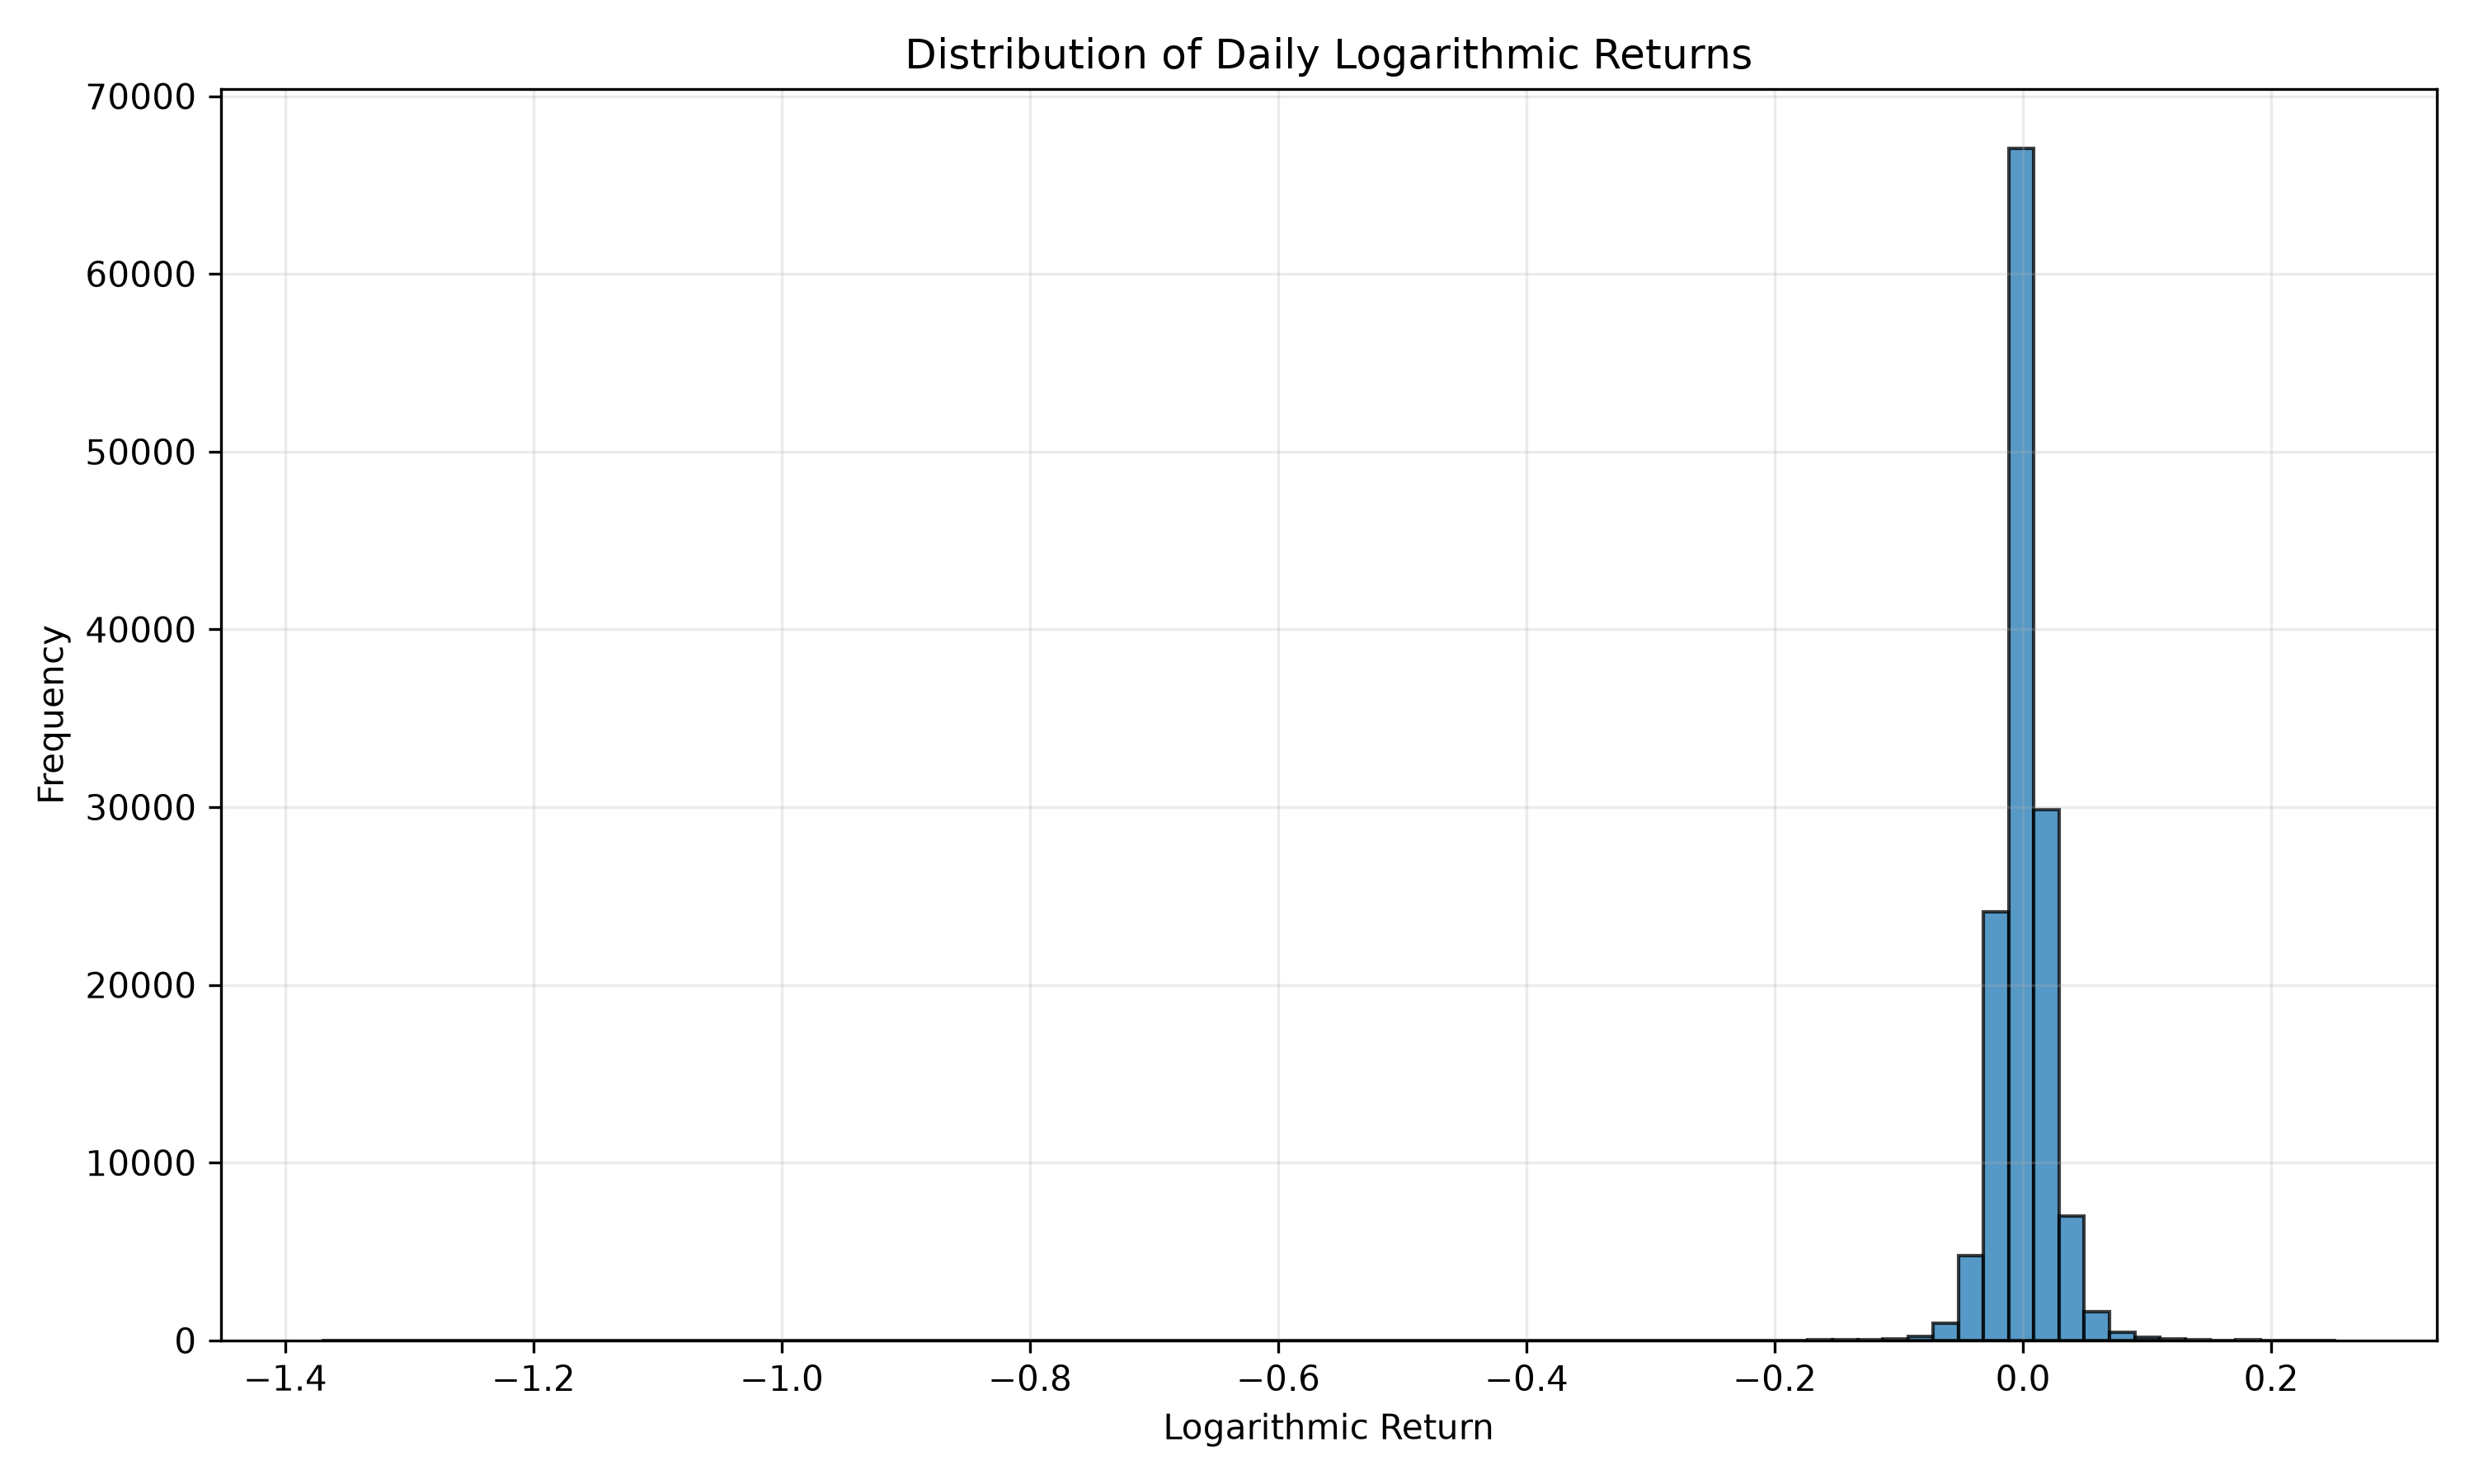
\includegraphics[width=0.70\textwidth]
    {overall_return_distribution.png}
    \caption{Distribution of Daily Logarithmic Returns}
    \label{fig:return_distribution}
\end{figure}

The histogram provides an overview of the return
distribution across the analysed companies.

\subsection{Pearson Correlation Heatmap}

Figure \ref{fig:correlation_heatmap} presents the
Pearson correlation matrix of the 184 companies.

The diagonal contains values equal to 1 because
each company is perfectly correlated with itself.

Most off-diagonal values show weak-to-moderate positive
relationships. Some company pairs exhibit stronger
positive correlations.

The heatmap provides a visual representation of
the relationships that are subsequently converted
into network edges.

\begin{figure}[H]
    \centering
    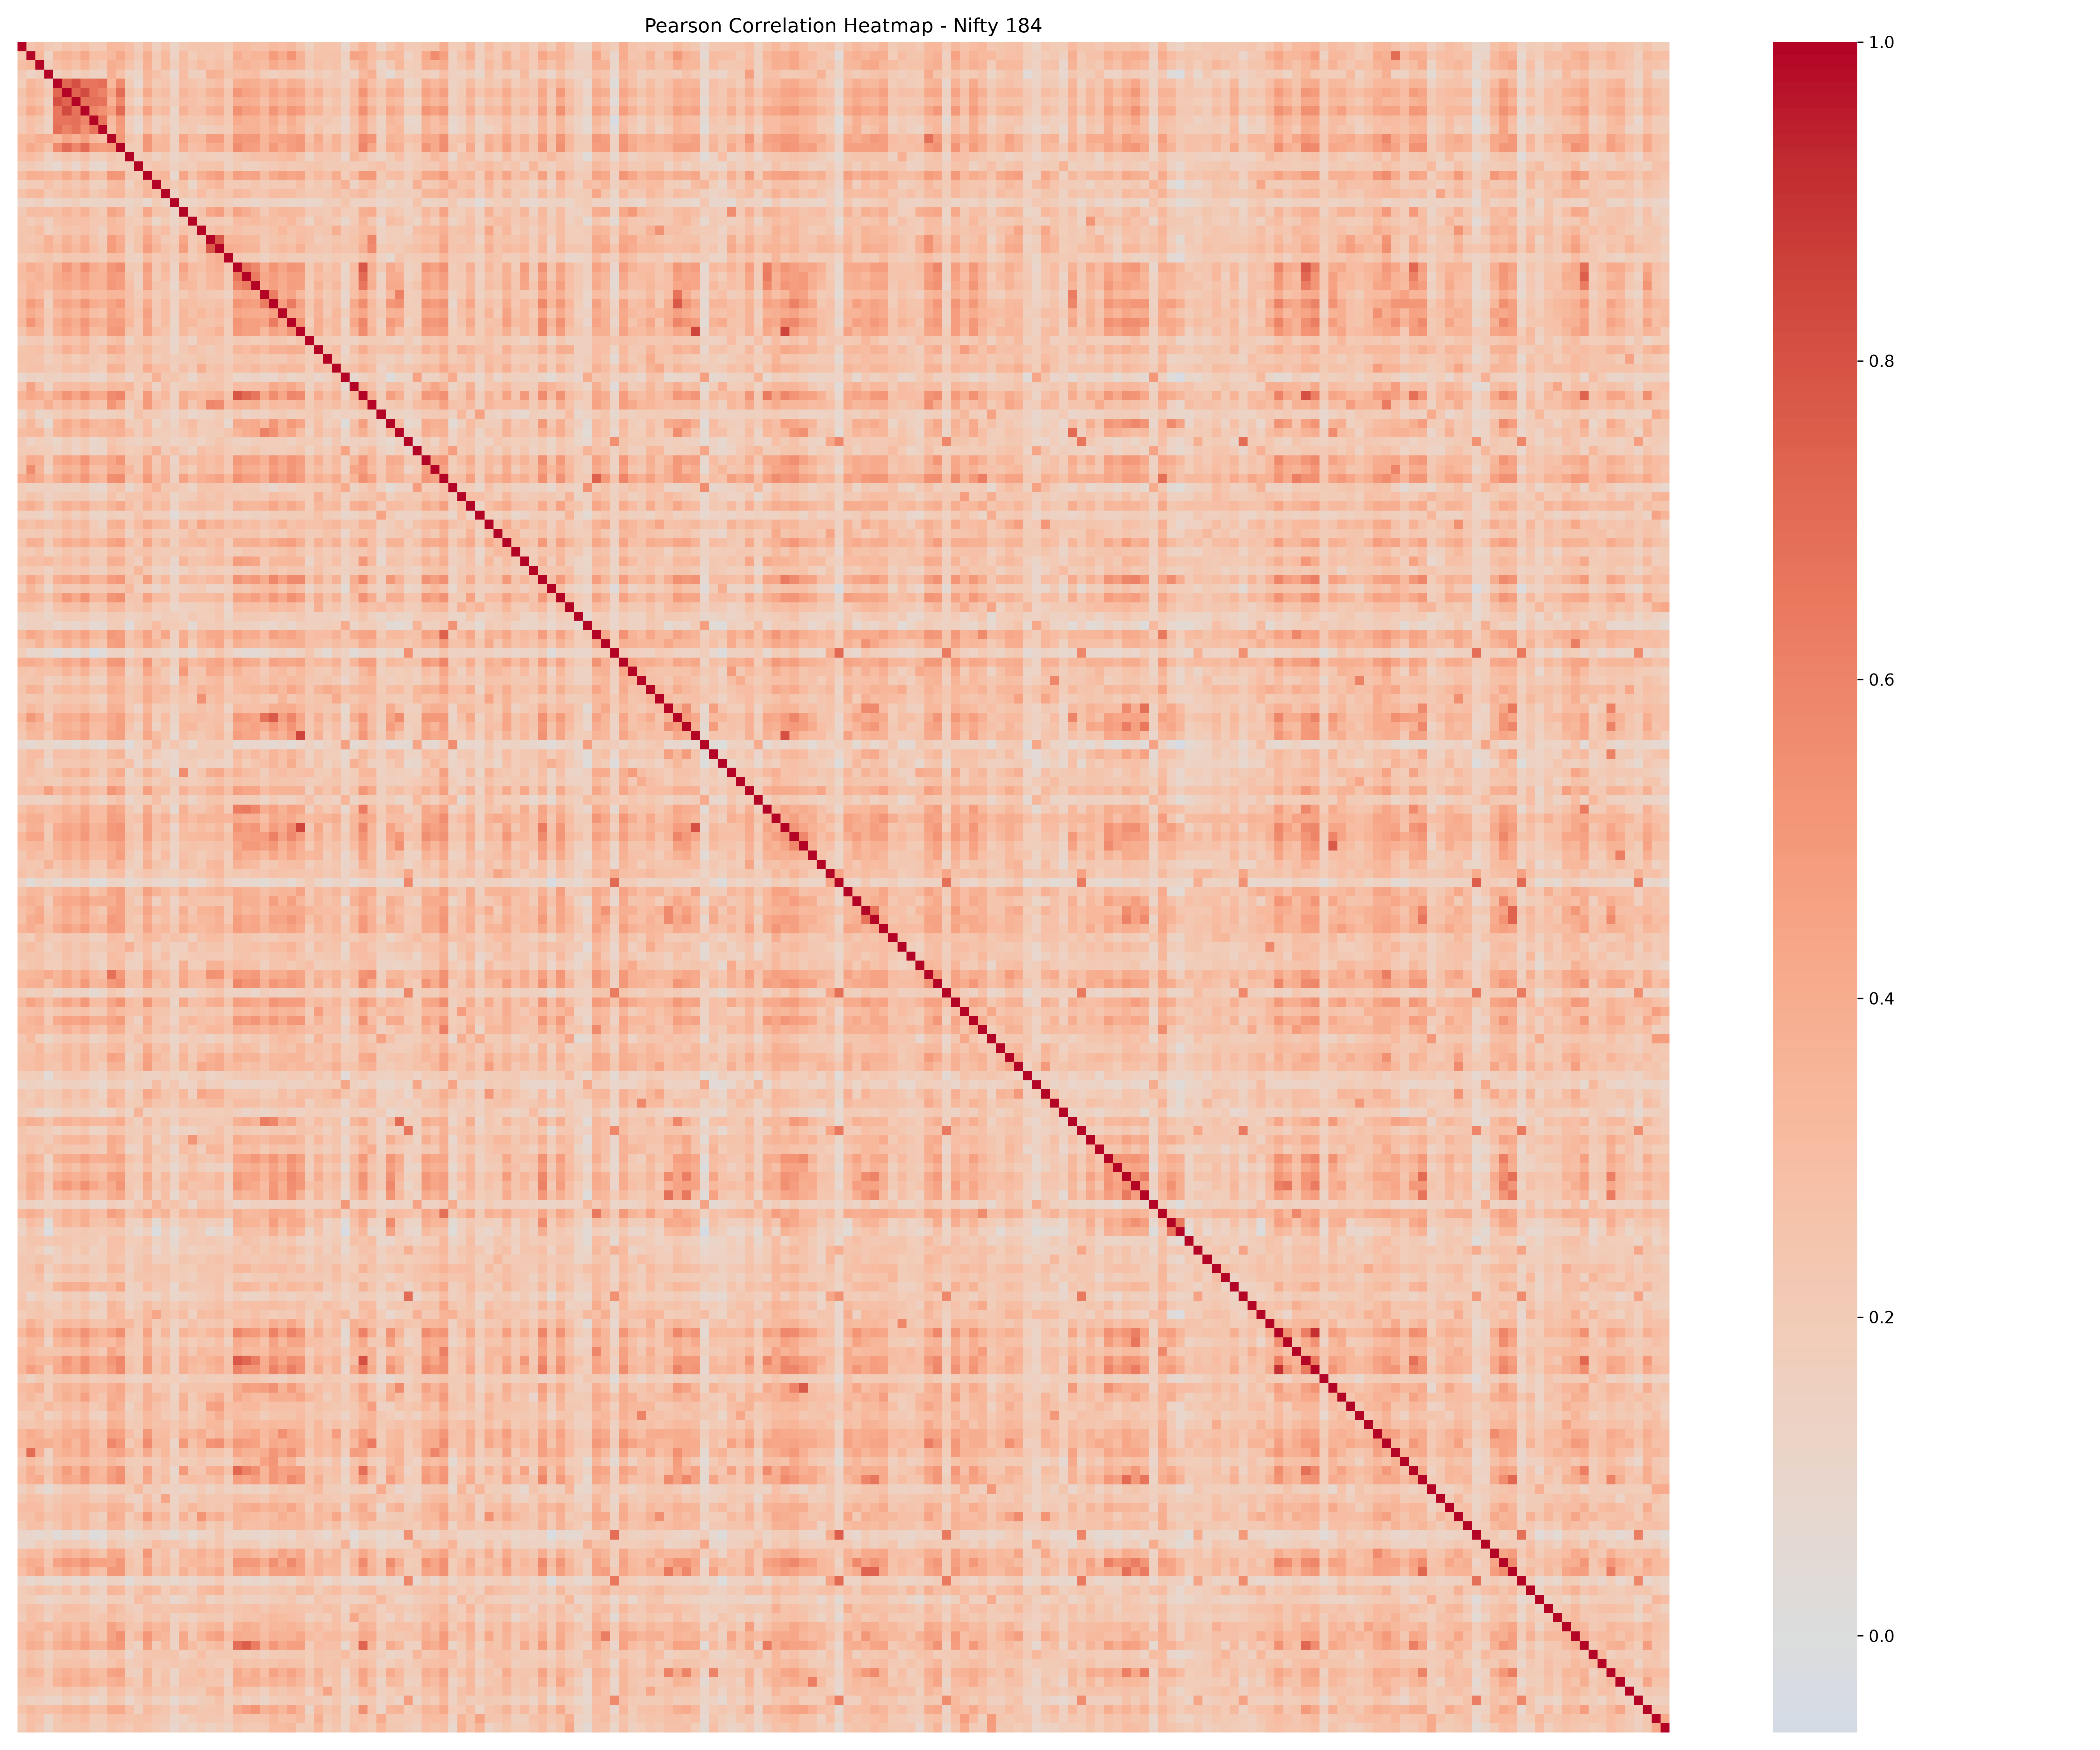
\includegraphics[width=0.65\textwidth]
    {correlation_heatmap.png}
    \caption{Pearson Correlation Heatmap of Nifty 184 Companies}
    \label{fig:correlation_heatmap}
\end{figure}

The mean pairwise correlation is approximately 0.2684.
This indicates a generally positive average relationship
among the analysed companies, although the strength
of the relationship varies considerably across pairs.

\subsection{Stock Market Network at Threshold 0.6}

The main network was constructed using a correlation
threshold of 0.6.

Two companies are connected only when their Pearson
correlation coefficient is at least 0.6.

The resulting network has the following properties:

\begin{table}[H]
\centering
\caption{Summary of the Stock Market Network at Threshold 0.6}
\label{tab:network_summary}
\begin{tabular}{lr}
\toprule
\textbf{Network Measure} & \textbf{Value}\\
\midrule
Number of Nodes & 184\\
Number of Edges & 126\\
Network Density & 0.0075\\
Connected Components & 122\\
Largest Component Size & 25\\
Average Degree & 1.3696\\
Average Clustering Coefficient & 0.1962\\
\bottomrule
\end{tabular}
\end{table}

The network density is calculated as:

\[
D=\frac{2(126)}{184(183)}
\]

\[
D\approx 0.0075
\]

The low density indicates that only a small proportion
of all possible company pairs are connected at this
correlation threshold.

Figure \ref{fig:stock_network} presents the visual
representation of the network.

\begin{figure}[H]
    \centering
    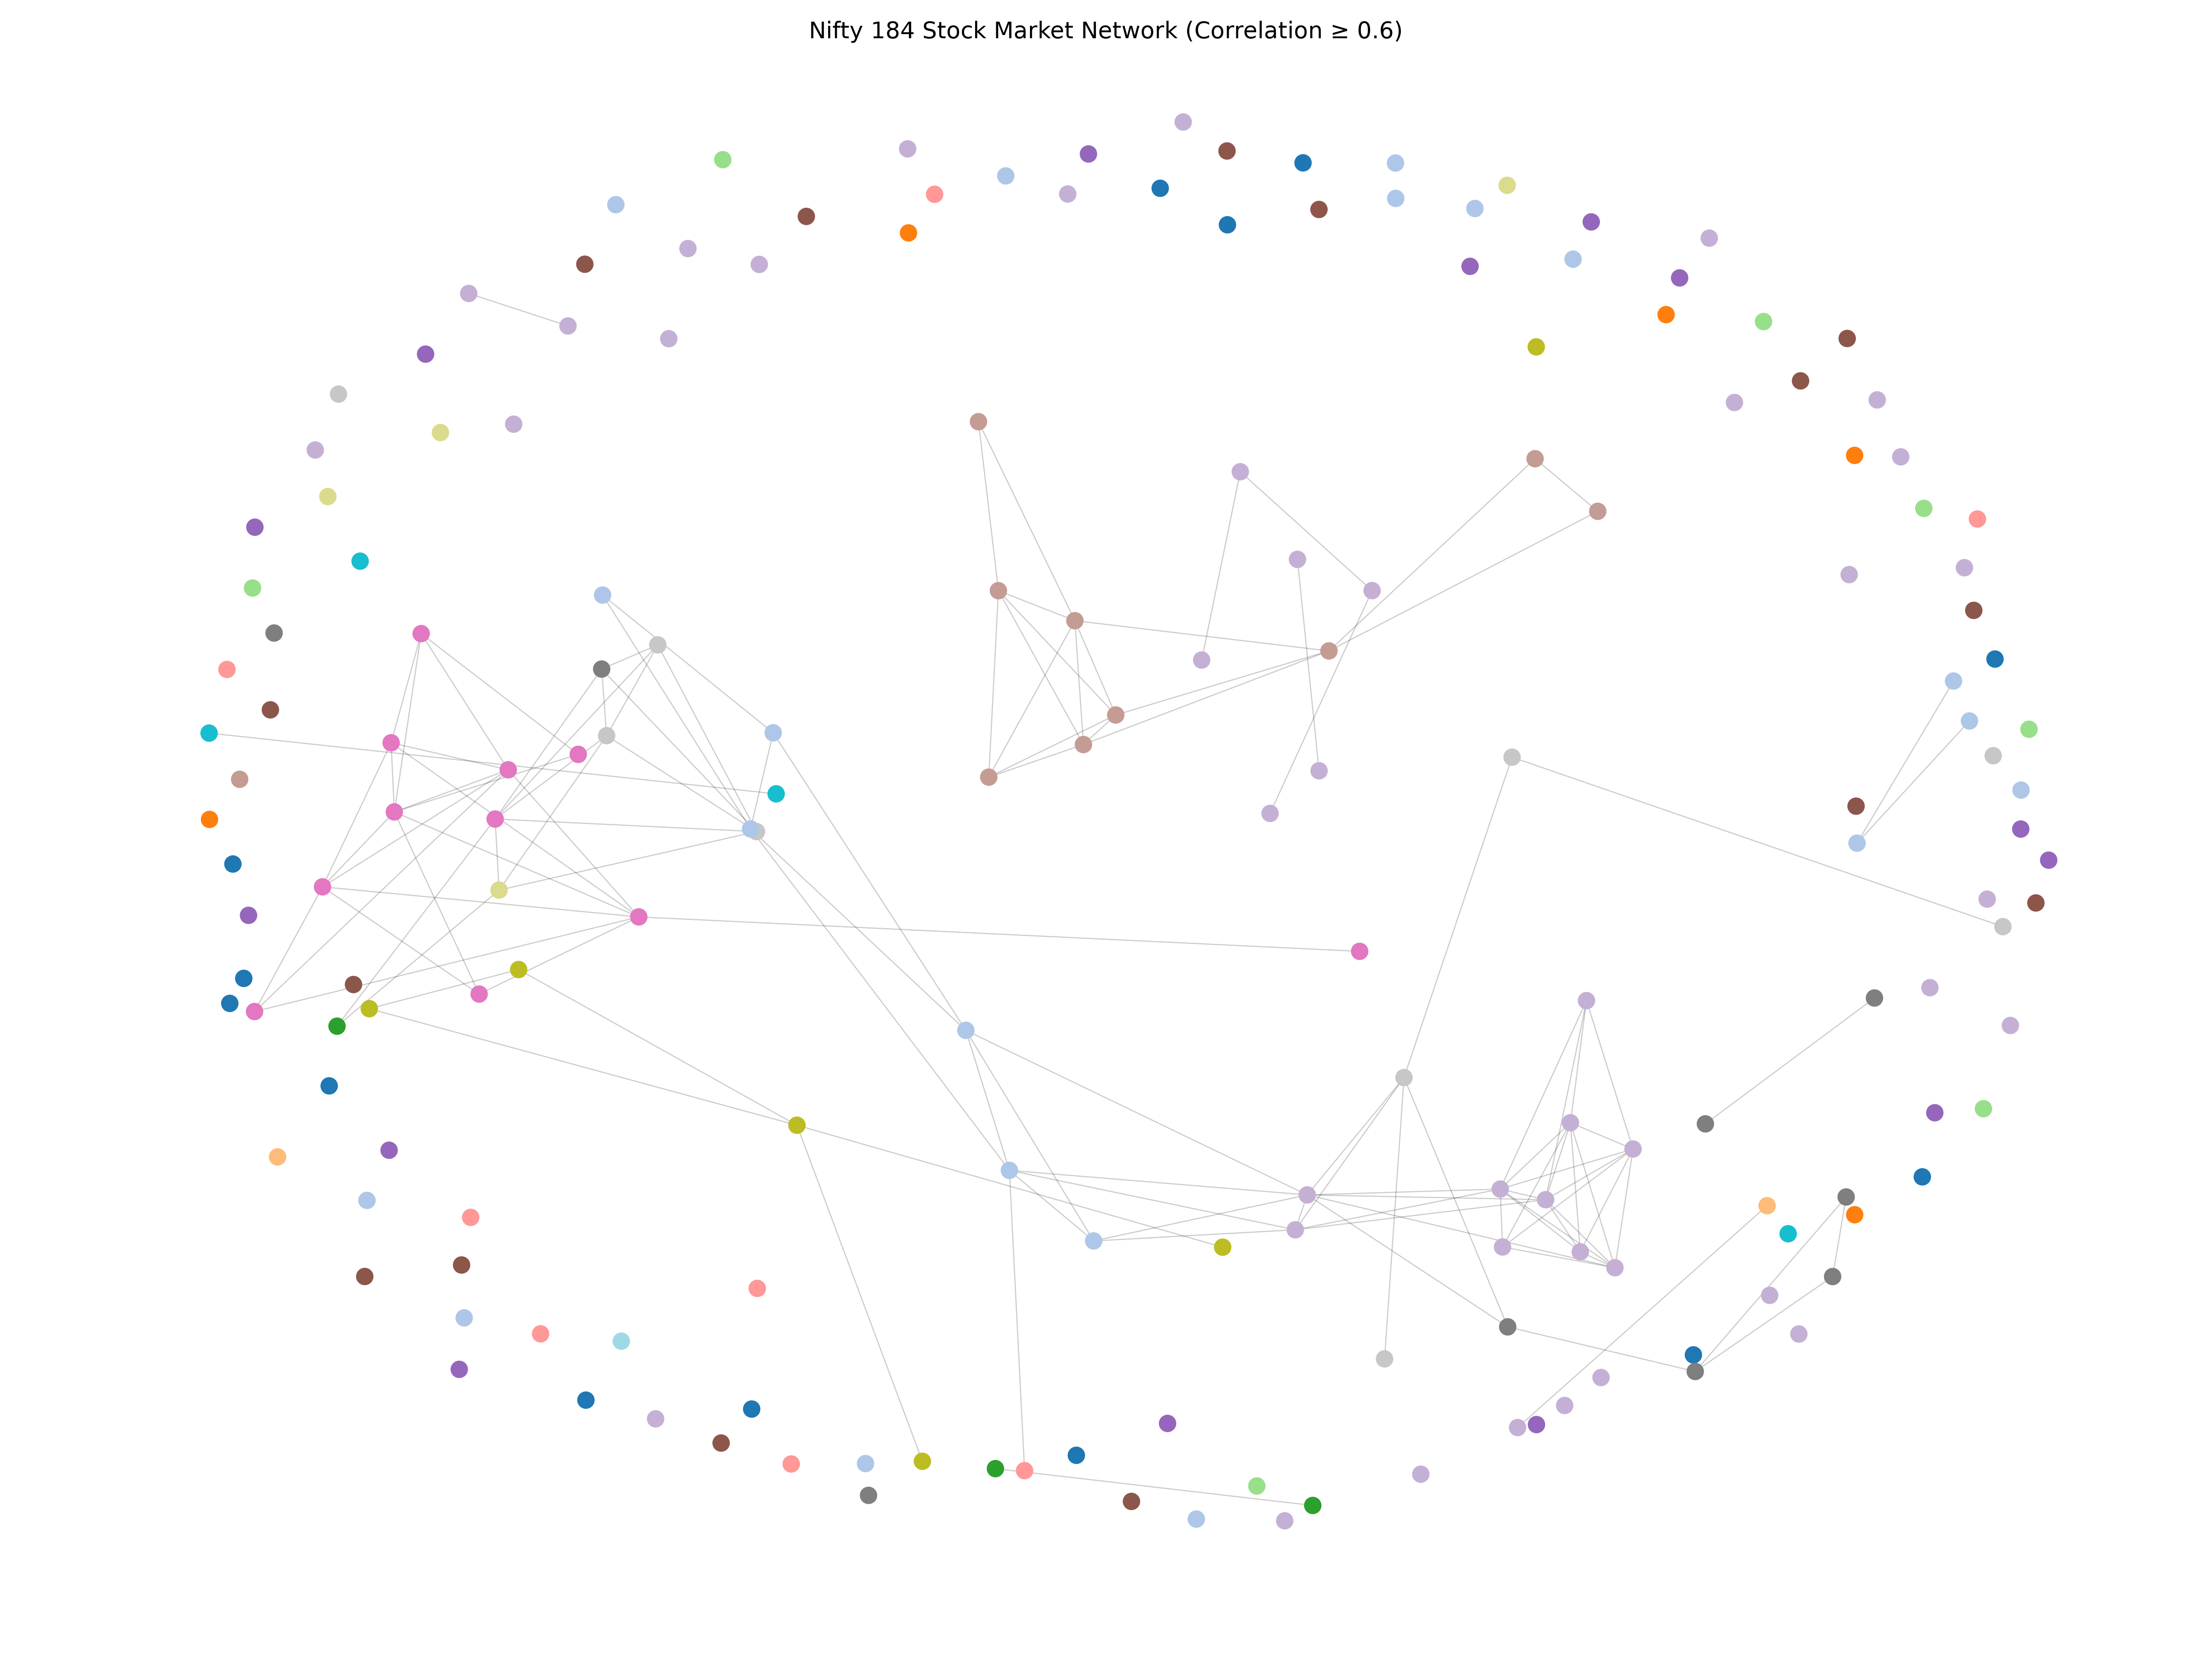
\includegraphics[width=0.95\textwidth]
    {nifty184_network_r06.png}
    \caption{Nifty 184 Stock Market Network at Correlation Threshold 0.6}
    \label{fig:stock_network}
\end{figure}

The network is highly fragmented. Many companies
remain isolated, while some groups form connected
clusters.

This indicates that strong positive return correlations
are concentrated among selected groups rather than
being distributed uniformly across the market.

\subsection{Degree Distribution}

Degree distribution describes the number of companies
having a particular number of connections.

It helps identify whether most companies have similar
connectivity or whether a small number of companies
have substantially more connections than others.

\subsubsection{Degree Distribution on Linear Scale}

Figure \ref{fig:degree_linear} presents the degree
distribution on a linear scale.

A large number of companies have degree zero.
This means that they do not have any other company
connected to them at the selected threshold of 0.6.

A smaller number of companies have one or more
connections. Only a few companies have relatively
high degrees.

\begin{figure}[H]
    \centering
    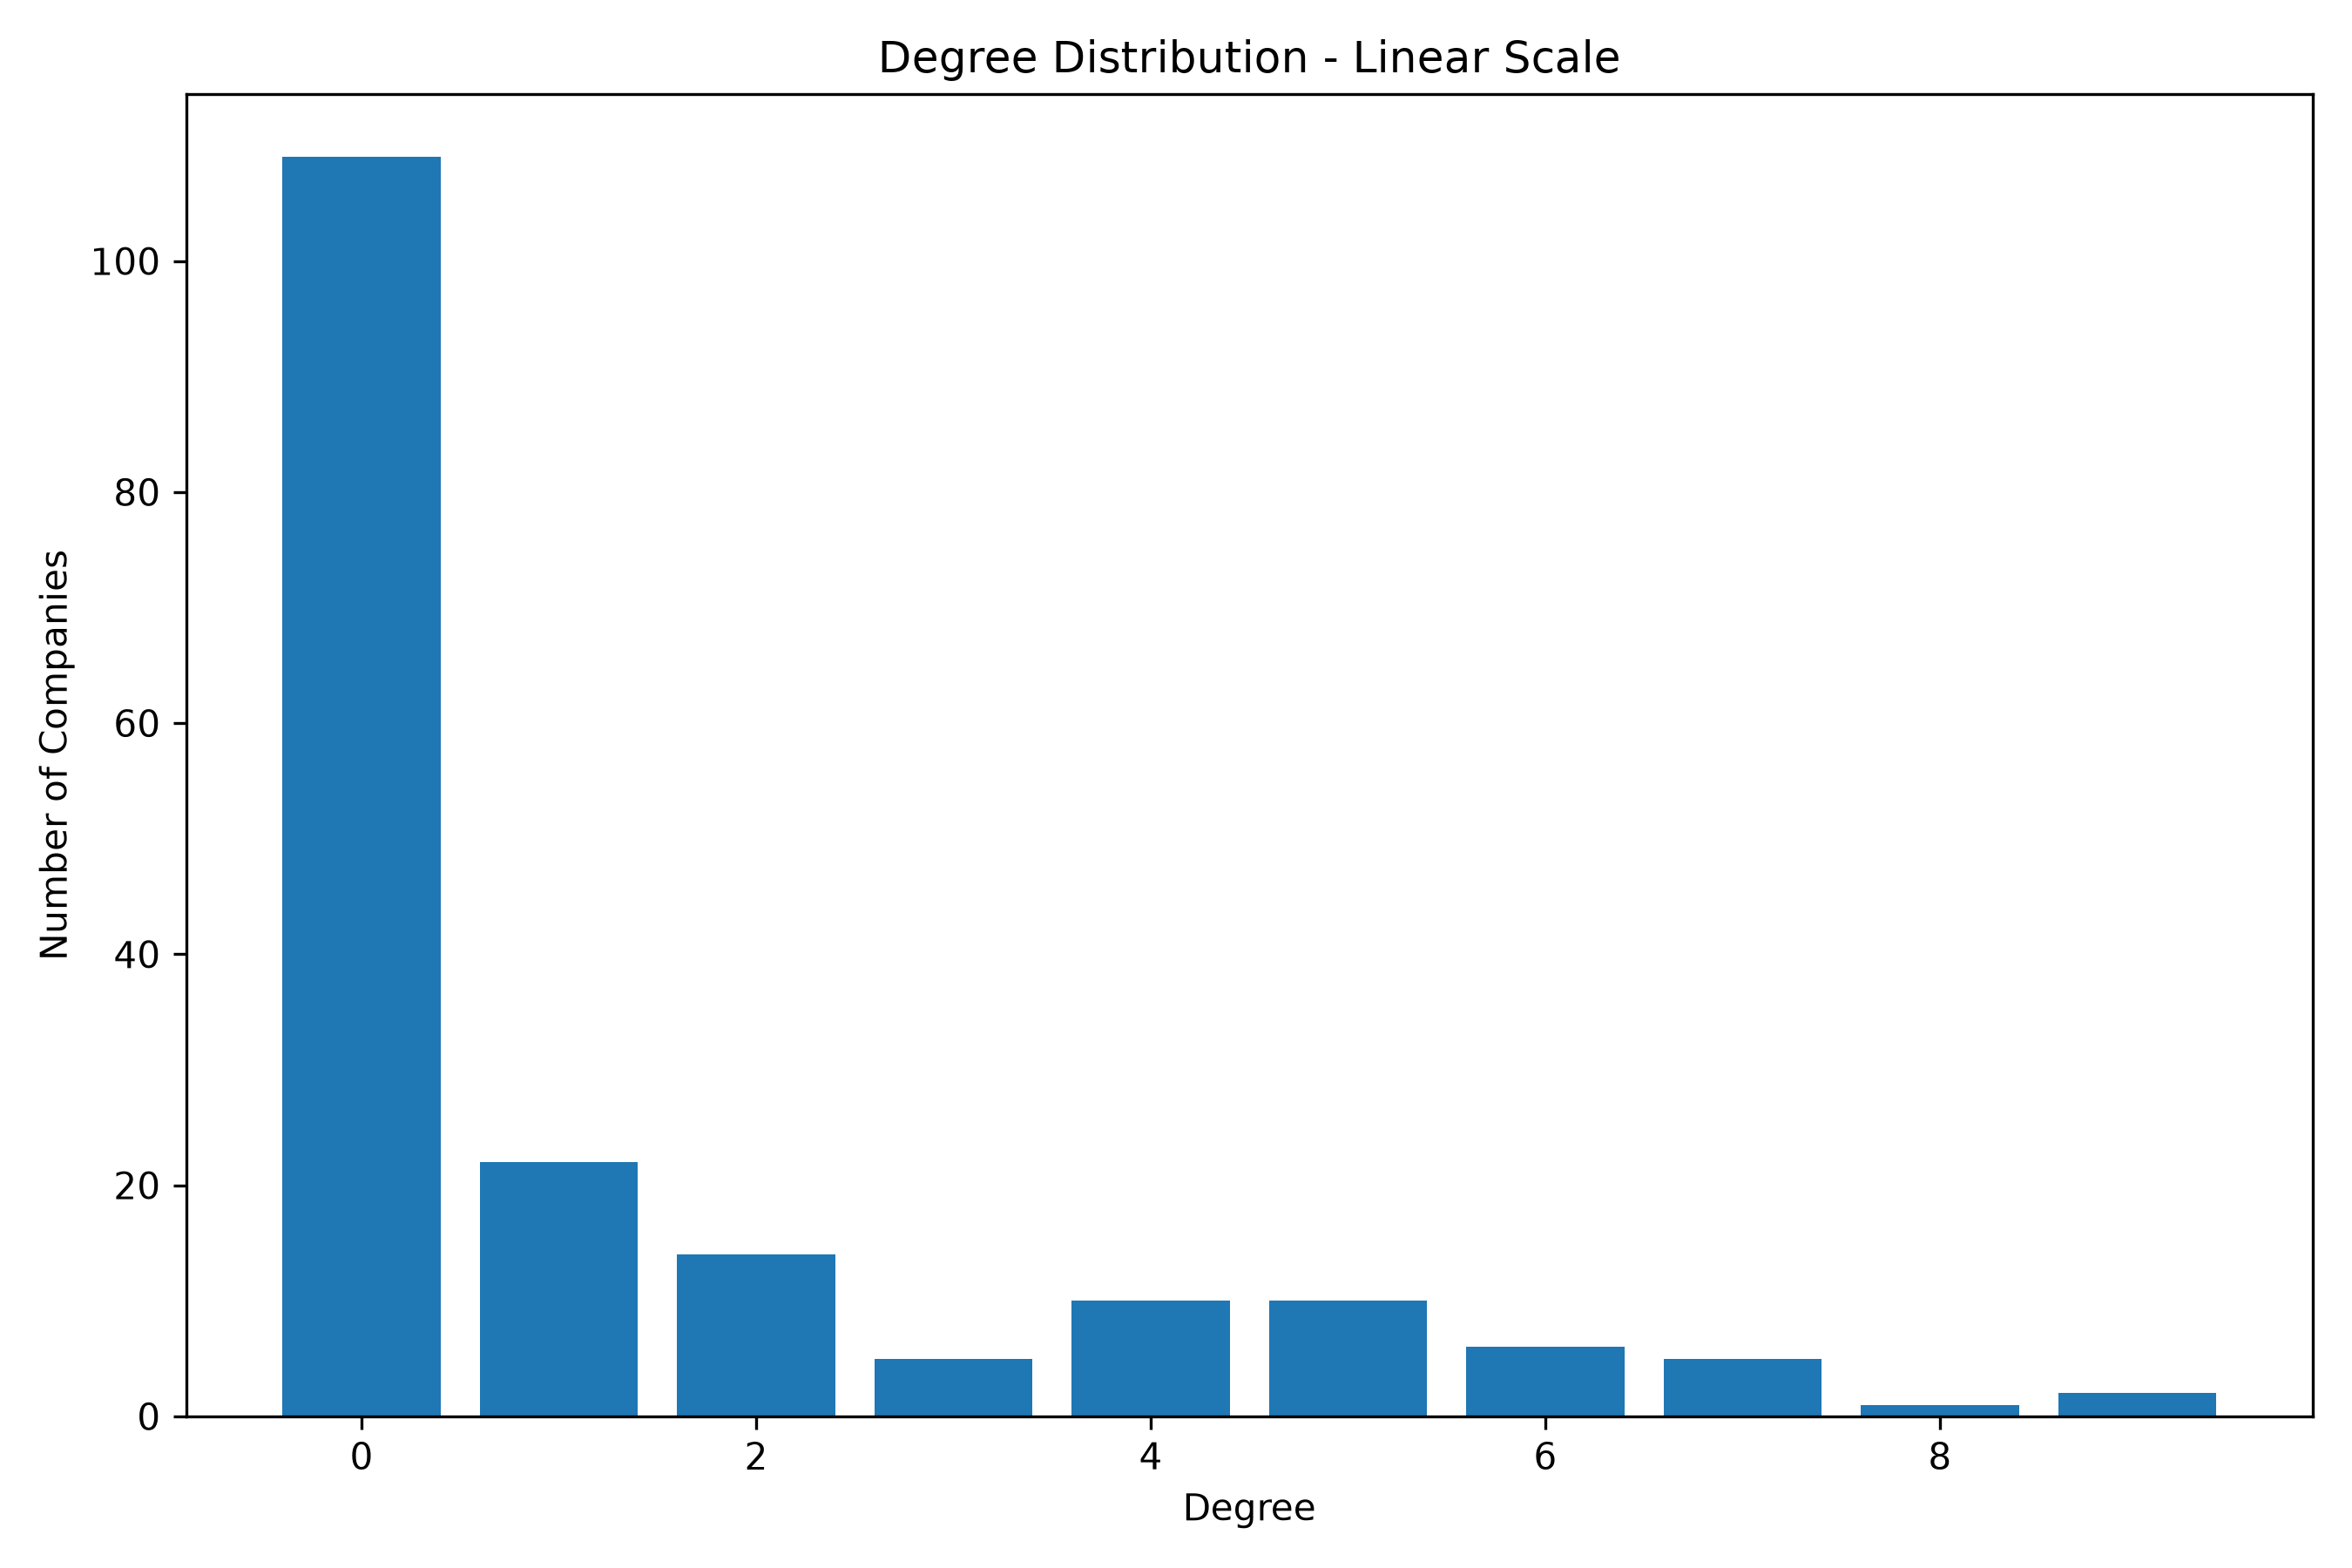
\includegraphics[width=0.85\textwidth]
    {degree_distribution_linear.png}
    \caption{Degree Distribution on Linear Scale}
    \label{fig:degree_linear}
\end{figure}

The distribution indicates that the network contains
many isolated nodes and a relatively small number
of connected companies.

\subsubsection{Degree Distribution on Log-Log Scale}

Figure \ref{fig:degree_loglog} presents the degree
distribution using logarithmic scales on both axes.

A log-log representation helps examine the distribution
of low- and high-degree nodes.

\begin{figure}[H]
    \centering
    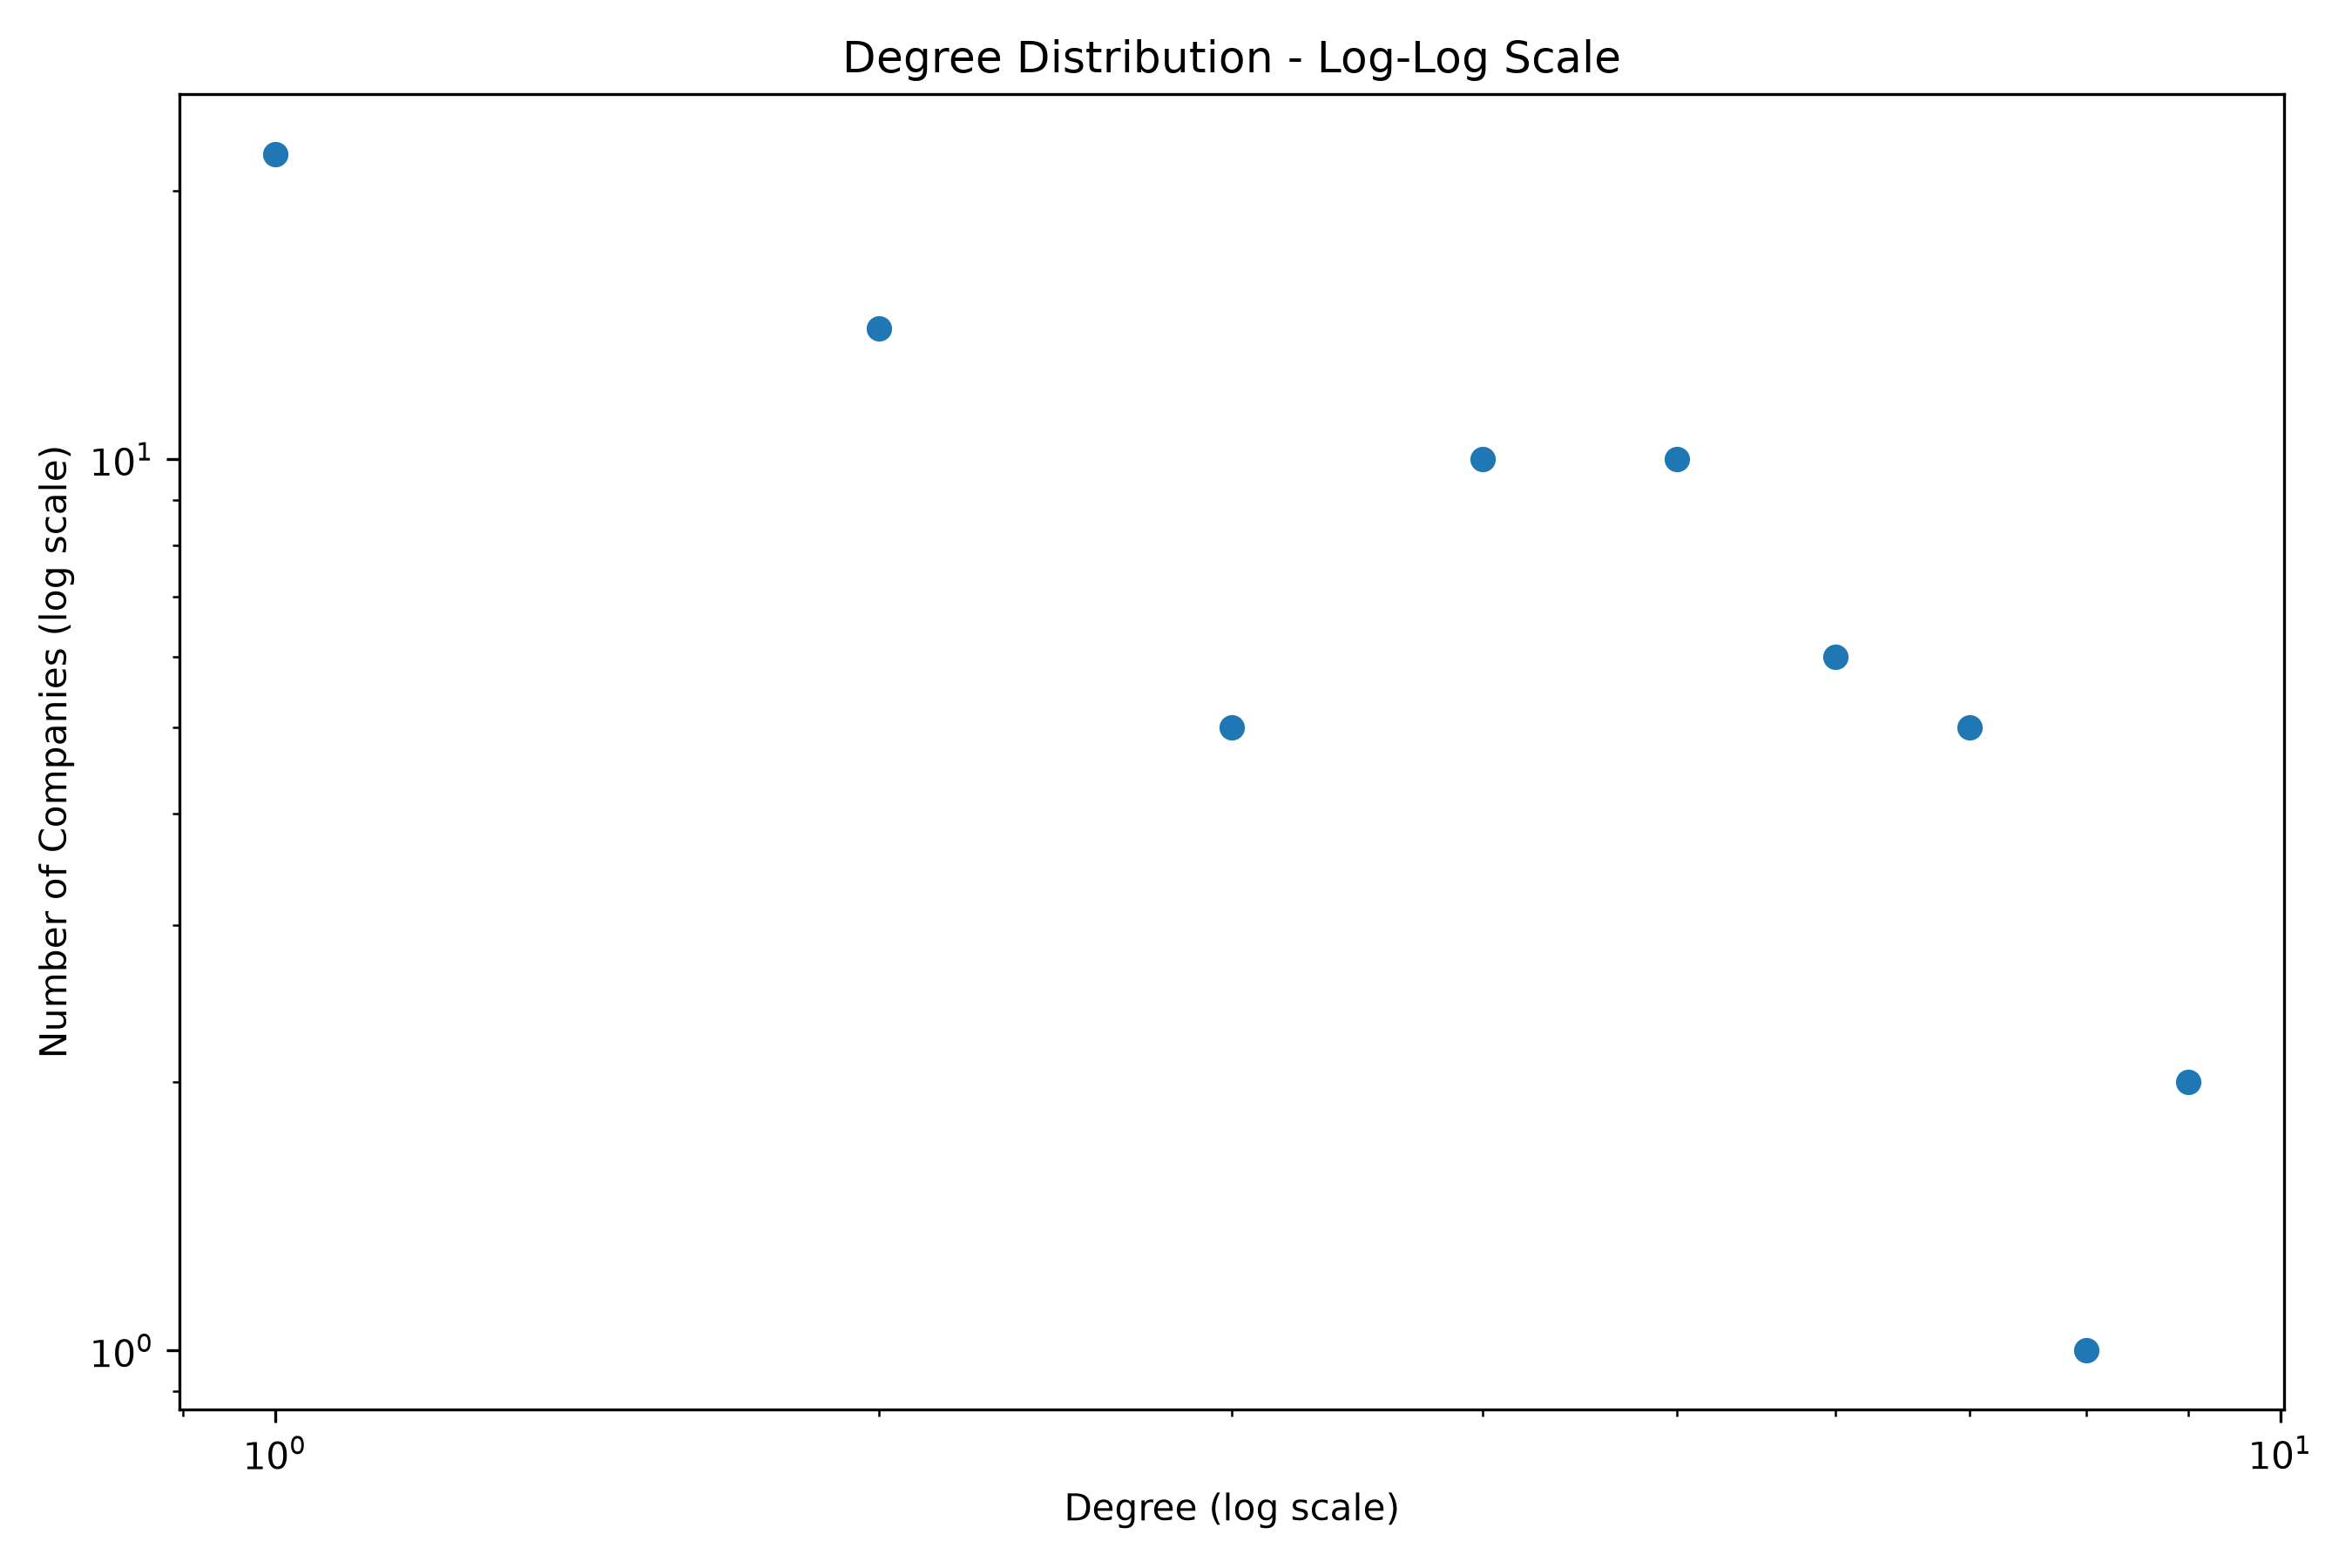
\includegraphics[width=0.85\textwidth]
    {degree_distribution_loglog.png}
    \caption{Degree Distribution on Log-Log Scale}
    \label{fig:degree_loglog}
\end{figure}

The distribution is concentrated at low degrees.
However, the limited number of distinct degree values
and the small number of high-degree nodes do not
provide sufficient evidence to establish a power-law
distribution.

Therefore, the degree distribution should be interpreted
as a sparse and uneven connectivity pattern rather than
as proof of a scale-free network.

\subsection{Centrality Analysis}

Centrality measures identify companies that occupy
important structural positions in the network.

Three centrality measures were examined:

\begin{itemize}
    \item Degree centrality.
    \item Betweenness centrality.
    \item Eigenvector centrality.
\end{itemize}

\subsubsection{Top 10 Companies by Degree Centrality}

Degree centrality identifies companies with the largest
number of direct connections.

\begin{table}[H]
\centering
\caption{Top 10 Companies by Degree Centrality}
\label{tab:degree_centrality}
\small
\begin{tabular}{cllr}
\toprule
\textbf{Rank} & \textbf{Company} & \textbf{Industry} &
\textbf{Centrality}\\
\midrule
1 & CANBK & Financial Services & 0.049180\\
2 & RECLTD & Financial Services & 0.049180\\
3 & PNB & Financial Services & 0.043716\\
4 & UNIONBANK & Financial Services & 0.038251\\
5 & BANKBARODA & Financial Services & 0.038251\\
6 & VEDL & Metals \& Mining & 0.038251\\
7 & BANKINDIA & Financial Services & 0.038251\\
8 & TATASTEEL & Metals \& Mining & 0.038251\\
9 & PFC & Financial Services & 0.032787\\
10 & BEL & Capital Goods & 0.032787\\
\bottomrule
\end{tabular}
\end{table}

CANBK and RECLTD have the highest degree centrality.
Both companies have the largest number of direct
connections in the network.

Financial Services companies appear frequently among
the top-ranked companies, indicating that several
companies in this sector have strong relationships
with other companies in the network.

\subsubsection{Top 10 Companies by Betweenness Centrality}

Betweenness centrality identifies companies that
occupy important connecting positions along shortest
paths between other companies.

\begin{table}[H]
\centering
\caption{Top 10 Companies by Betweenness Centrality}
\label{tab:betweenness}
\small
\begin{tabular}{cllr}
\toprule
\textbf{Rank} & \textbf{Company} & \textbf{Industry} &
\textbf{Centrality}\\
\midrule
1 & RECLTD & Financial Services & 0.008765\\
2 & NTPC & Power & 0.004023\\
3 & GAIL & Oil Gas \& Consumable Fuels & 0.003783\\
4 & BEL & Capital Goods & 0.002648\\
5 & IOC & Oil Gas \& Consumable Fuels & 0.002642\\
6 & CANBK & Financial Services & 0.002379\\
7 & HAL & Capital Goods & 0.002251\\
8 & PFC & Financial Services & 0.001979\\
9 & PNB & Financial Services & 0.001708\\
10 & TATAPOWER & Power & 0.001381\\
\bottomrule
\end{tabular}
\end{table}

RECLTD has the highest betweenness centrality.
This suggests that it occupies an important connecting
position between different parts of the network.

Companies from sectors such as Power, Capital Goods
and Oil Gas also appear in the top rankings.

\subsubsection{Top 10 Companies by Eigenvector Centrality}

Eigenvector centrality considers not only the number
of connections but also the importance of the connected
companies.

\begin{table}[H]
\centering
\caption{Top 10 Companies by Eigenvector Centrality}
\label{tab:eigenvector}
\small
\begin{tabular}{cllr}
\toprule
\textbf{Rank} & \textbf{Company} & \textbf{Industry} &
\textbf{Centrality}\\
\midrule
1 & CANBK & Financial Services & 0.404894\\
2 & PNB & Financial Services & 0.375222\\
3 & BANKBARODA & Financial Services & 0.346269\\
4 & BANKINDIA & Financial Services & 0.339388\\
5 & UNIONBANK & Financial Services & 0.339388\\
6 & SBIN & Financial Services & 0.279441\\
7 & RECLTD & Financial Services & 0.277176\\
8 & MAHABANK & Financial Services & 0.225838\\
9 & INDIANB & Financial Services & 0.221356\\
10 & PFC & Financial Services & 0.211499\\
\bottomrule
\end{tabular}
\end{table}

CANBK has the highest eigenvector centrality.
This indicates that it is connected to other companies
that also occupy relatively important positions.

Financial Services companies dominate this ranking.

\subsubsection{Comparison of Centrality Measures}

The three centrality measures provide different
perspectives on the network.

\begin{itemize}
    \item Degree centrality identifies companies with
    the highest number of direct connections.

    \item Betweenness centrality identifies companies
    that connect different parts of the network.

    \item Eigenvector centrality identifies companies
    connected to other important companies.
\end{itemize}

RECLTD performs strongly in both degree and betweenness
centrality, while CANBK ranks highest in degree and
eigenvector centrality.

These measures describe structural importance within
the constructed network. They should not be interpreted
as indicators of future stock performance or investment
recommendations.

\subsection{Clustering Coefficient}

The average clustering coefficient of the network is
0.1962.

The clustering coefficient measures the extent to
which the neighbours of a company are connected
to one another.

A value of 0.1962 indicates a modest level of local
triangle formation in the network.

This means that some groups of companies have
interconnected relationships, but clustering is
not uniformly strong across the entire network.

\subsection{Sector Homophily}

Sector homophily examines whether companies belonging
to the same industry sector tend to be connected
to one another.

The analysis compares the industry classification
of both endpoints of every network edge.

\begin{table}[H]
\centering
\caption{Sector Homophily Results}
\label{tab:homophily}
\begin{tabular}{lr}
\toprule
\textbf{Measure} & \textbf{Value}\\
\midrule
Total Edges & 126\\
Same-Sector Edges & 103\\
Different-Sector Edges & 23\\
Same-Sector Edge Percentage & 81.75\%\\
Sector Assortativity & 0.7774\\
\bottomrule
\end{tabular}
\end{table}

The same-sector edge percentage is calculated as:

\[
H=\frac{103}{126}\times 100
\]

\[
H\approx 81.75\%
\]

Approximately 81.75\% of the network edges connect
companies belonging to the same industry sector.

The sector assortativity coefficient is 0.7774.
Its positive value indicates strong assortative mixing
by industry sector.

This suggests that companies operating in similar
industries tend to have stronger return correlations
than companies belonging to different sectors.

% =================================================
\section{Threshold Sensitivity Analysis}
% =================================================

The structure of a correlation-based network depends
on the threshold used to create edges.

A lower threshold allows more company pairs to become
connected, while a higher threshold retains only
stronger relationships.

To examine this effect, four thresholds were studied:

\[
r=0.5,\quad 0.6,\quad 0.7,\quad 0.8
\]

For each threshold, the following measures were examined:

\begin{itemize}
    \item Number of edges.
    \item Size of the largest connected component.
    \item Average path length within the largest connected component.
\end{itemize}

\subsection{Threshold vs Number of Edges}

Figure \ref{fig:threshold_edges} presents the relationship
between the correlation threshold and the number of edges.

\begin{figure}[H]
    \centering
    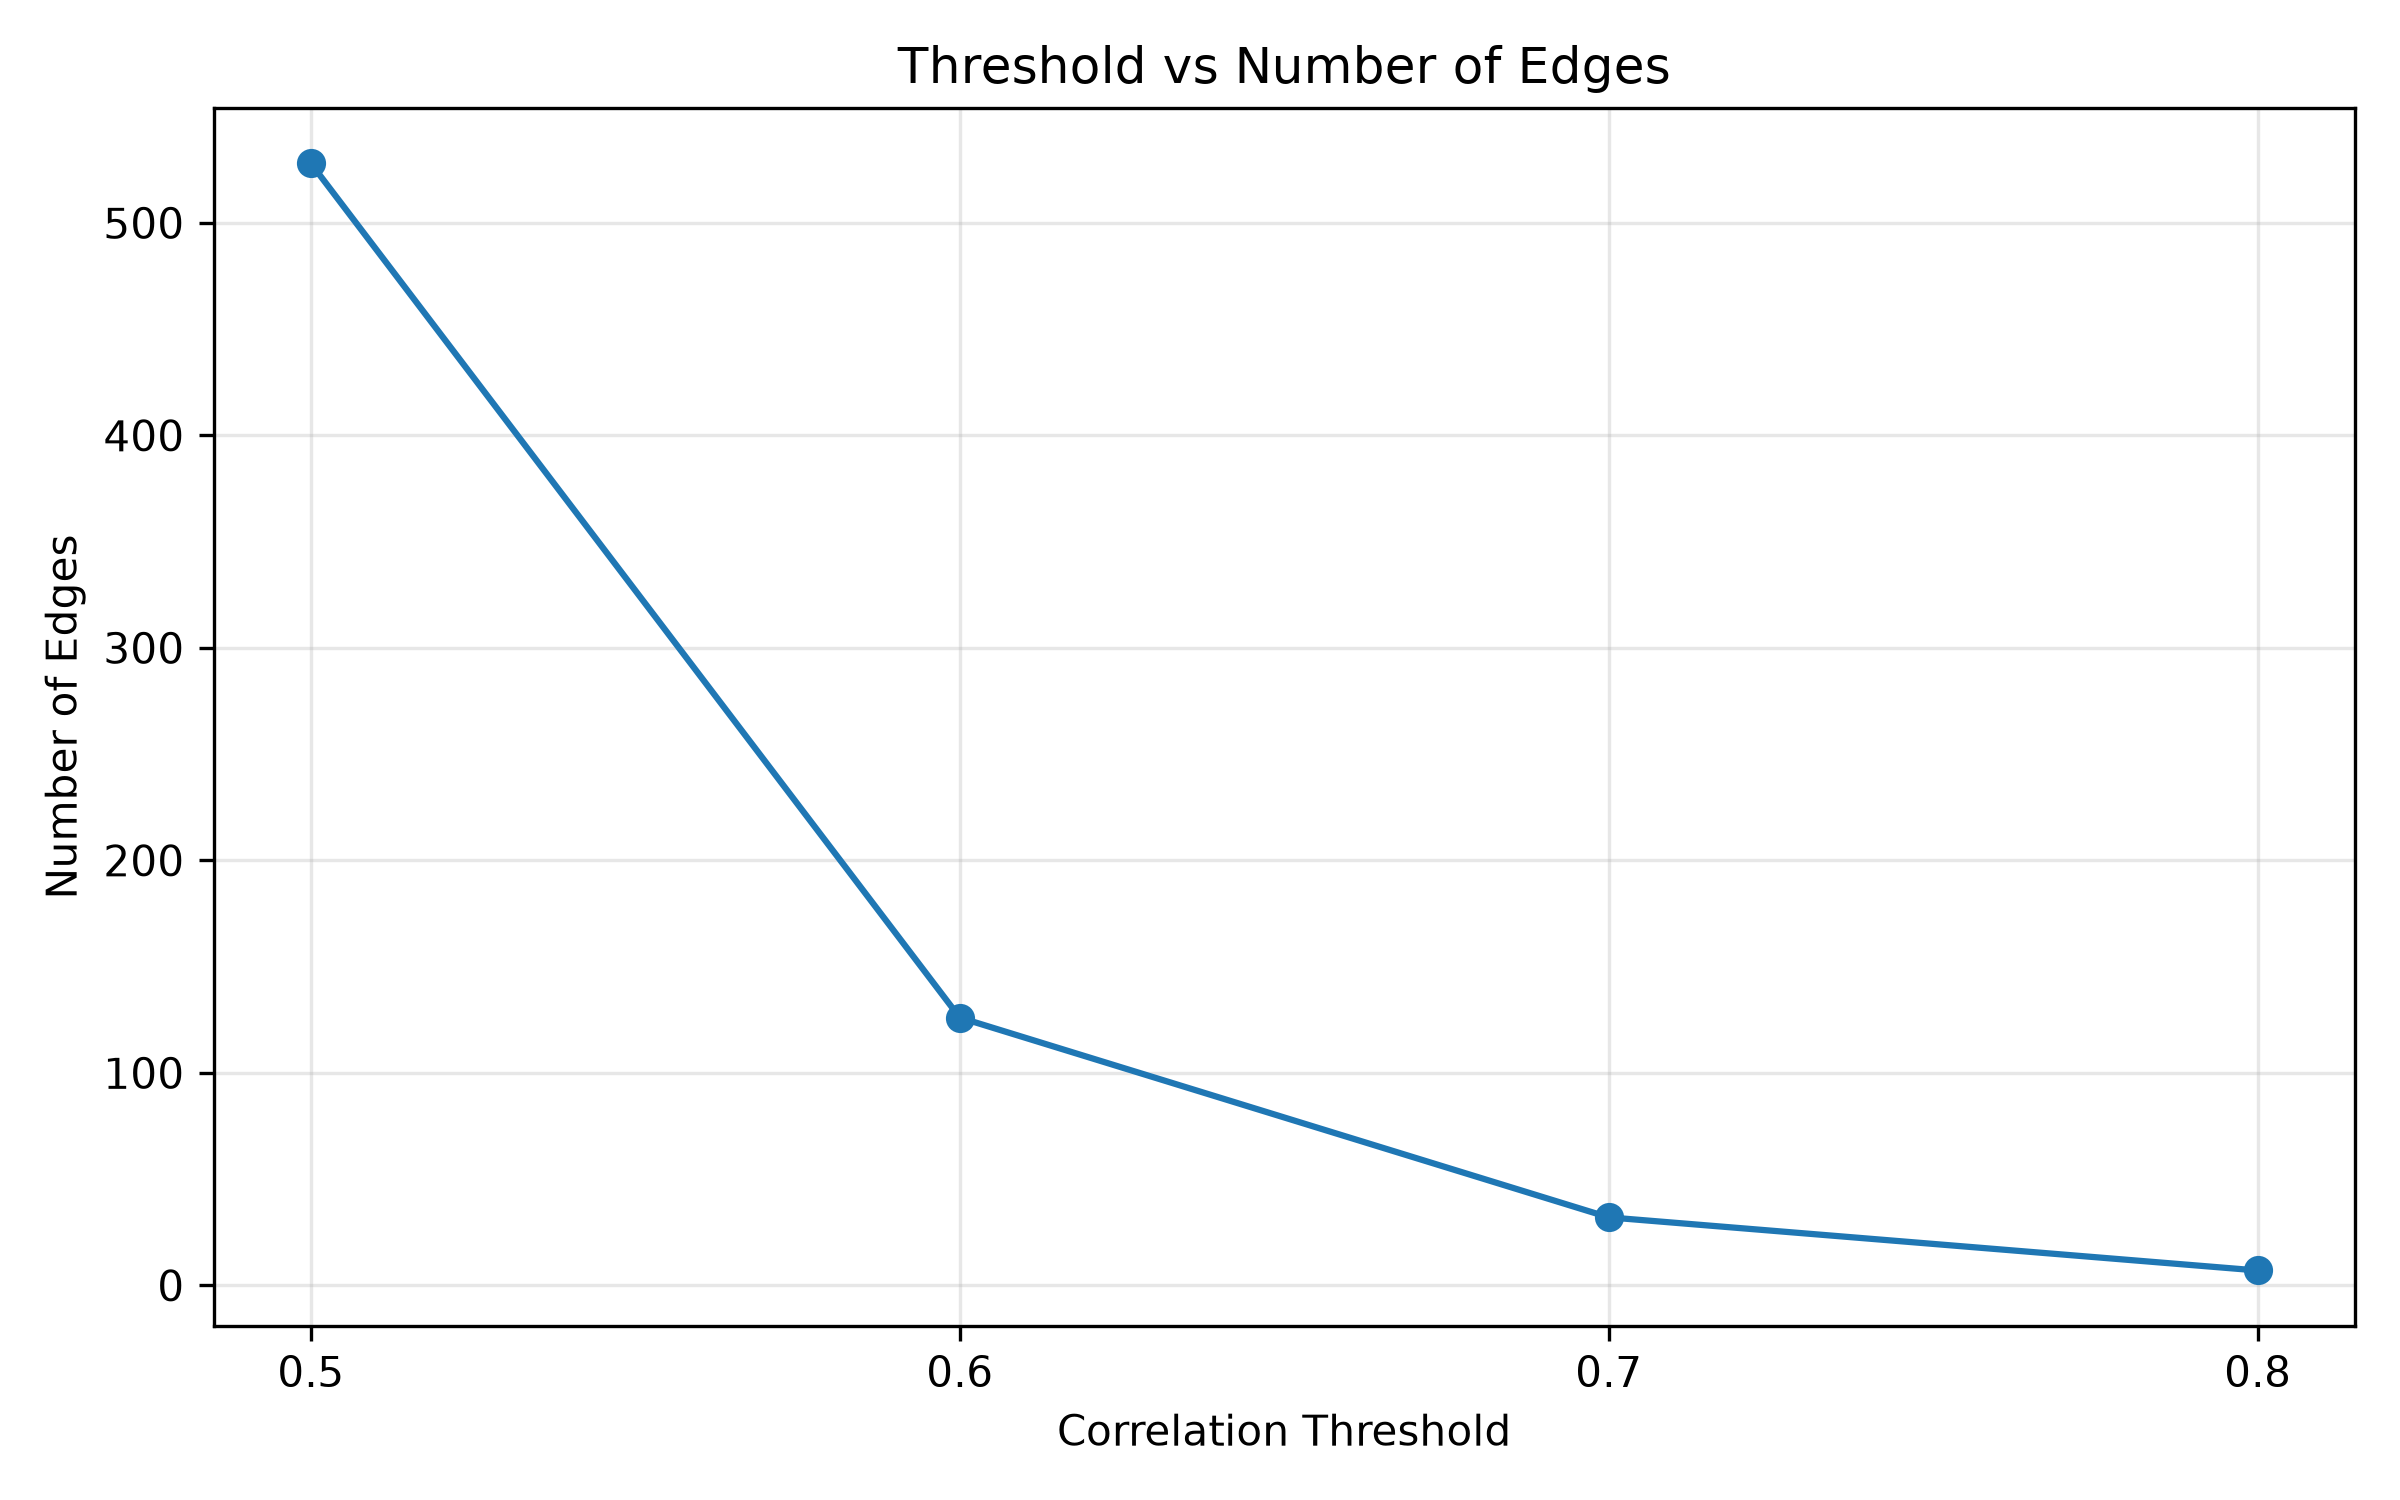
\includegraphics[width=0.85\textwidth]
    {threshold_vs_edges.png}
    \caption{Effect of Correlation Threshold on Number of Edges}
    \label{fig:threshold_edges}
\end{figure}

The number of edges decreases sharply as the threshold
increases.

At a threshold of 0.5, the network contains 528 edges.
When the threshold increases to 0.6, the number of edges
falls to 126.

At thresholds of 0.7 and 0.8, only 32 and 7 edges
remain respectively.

This demonstrates that the number of strong
correlations is much smaller than the number of
moderate correlations.

\subsection{Threshold vs Giant Component Size}

The giant component is the largest connected group
of nodes in a network.

Figure \ref{fig:threshold_giant} shows how the size
of the largest connected component changes as the
correlation threshold increases.

\begin{figure}[H]
    \centering
    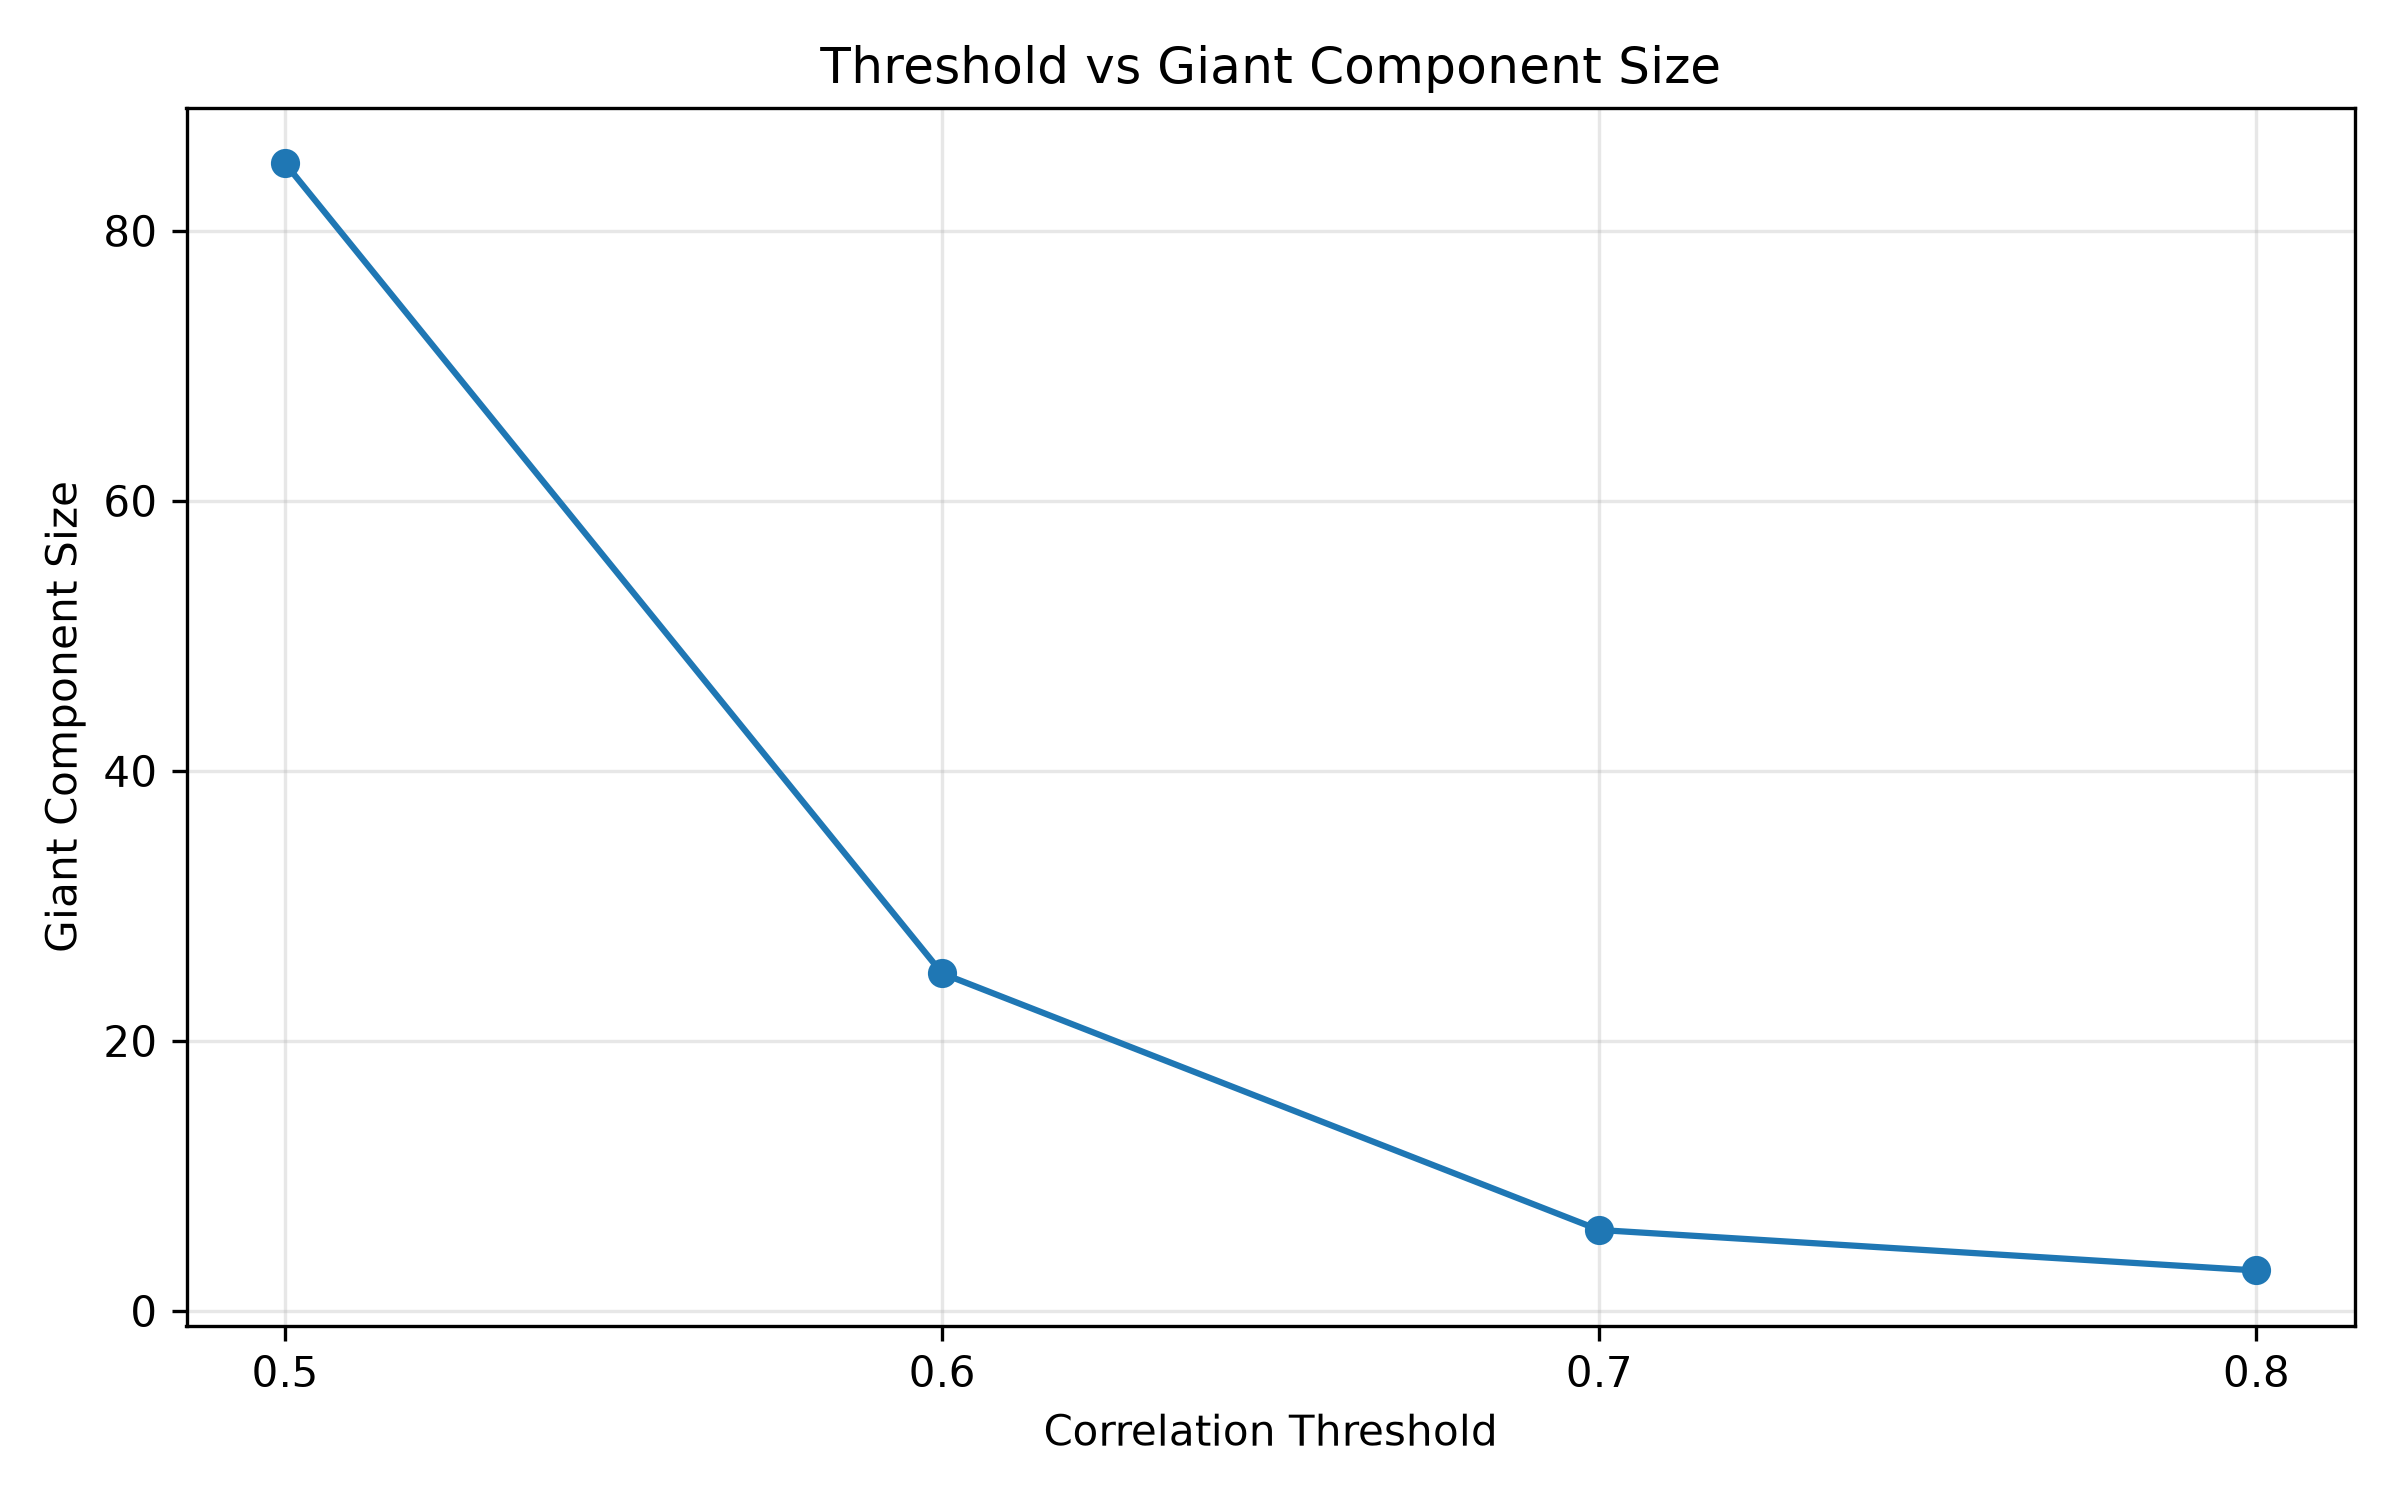
\includegraphics[width=0.85\textwidth]
    {threshold_vs_giant_component.png}
    \caption{Effect of Correlation Threshold on Giant Component Size}
    \label{fig:threshold_giant}
\end{figure}

At a threshold of 0.5, the largest connected component
contains 85 companies.

At a threshold of 0.6, it contains 25 companies.
The size further decreases to 6 at 0.7 and 3 at 0.8.

The reduction indicates that increasing the minimum
correlation requirement breaks the network into
smaller connected groups.

\subsection{Threshold vs Average Path Length}

Average path length measures the average shortest
distance between nodes within a connected component.

Since the complete network is disconnected, the
average path length is considered within the largest
connected component.

Figure \ref{fig:threshold_path} presents the
relationship between the threshold and average
path length.

\begin{figure}[H]
    \centering
    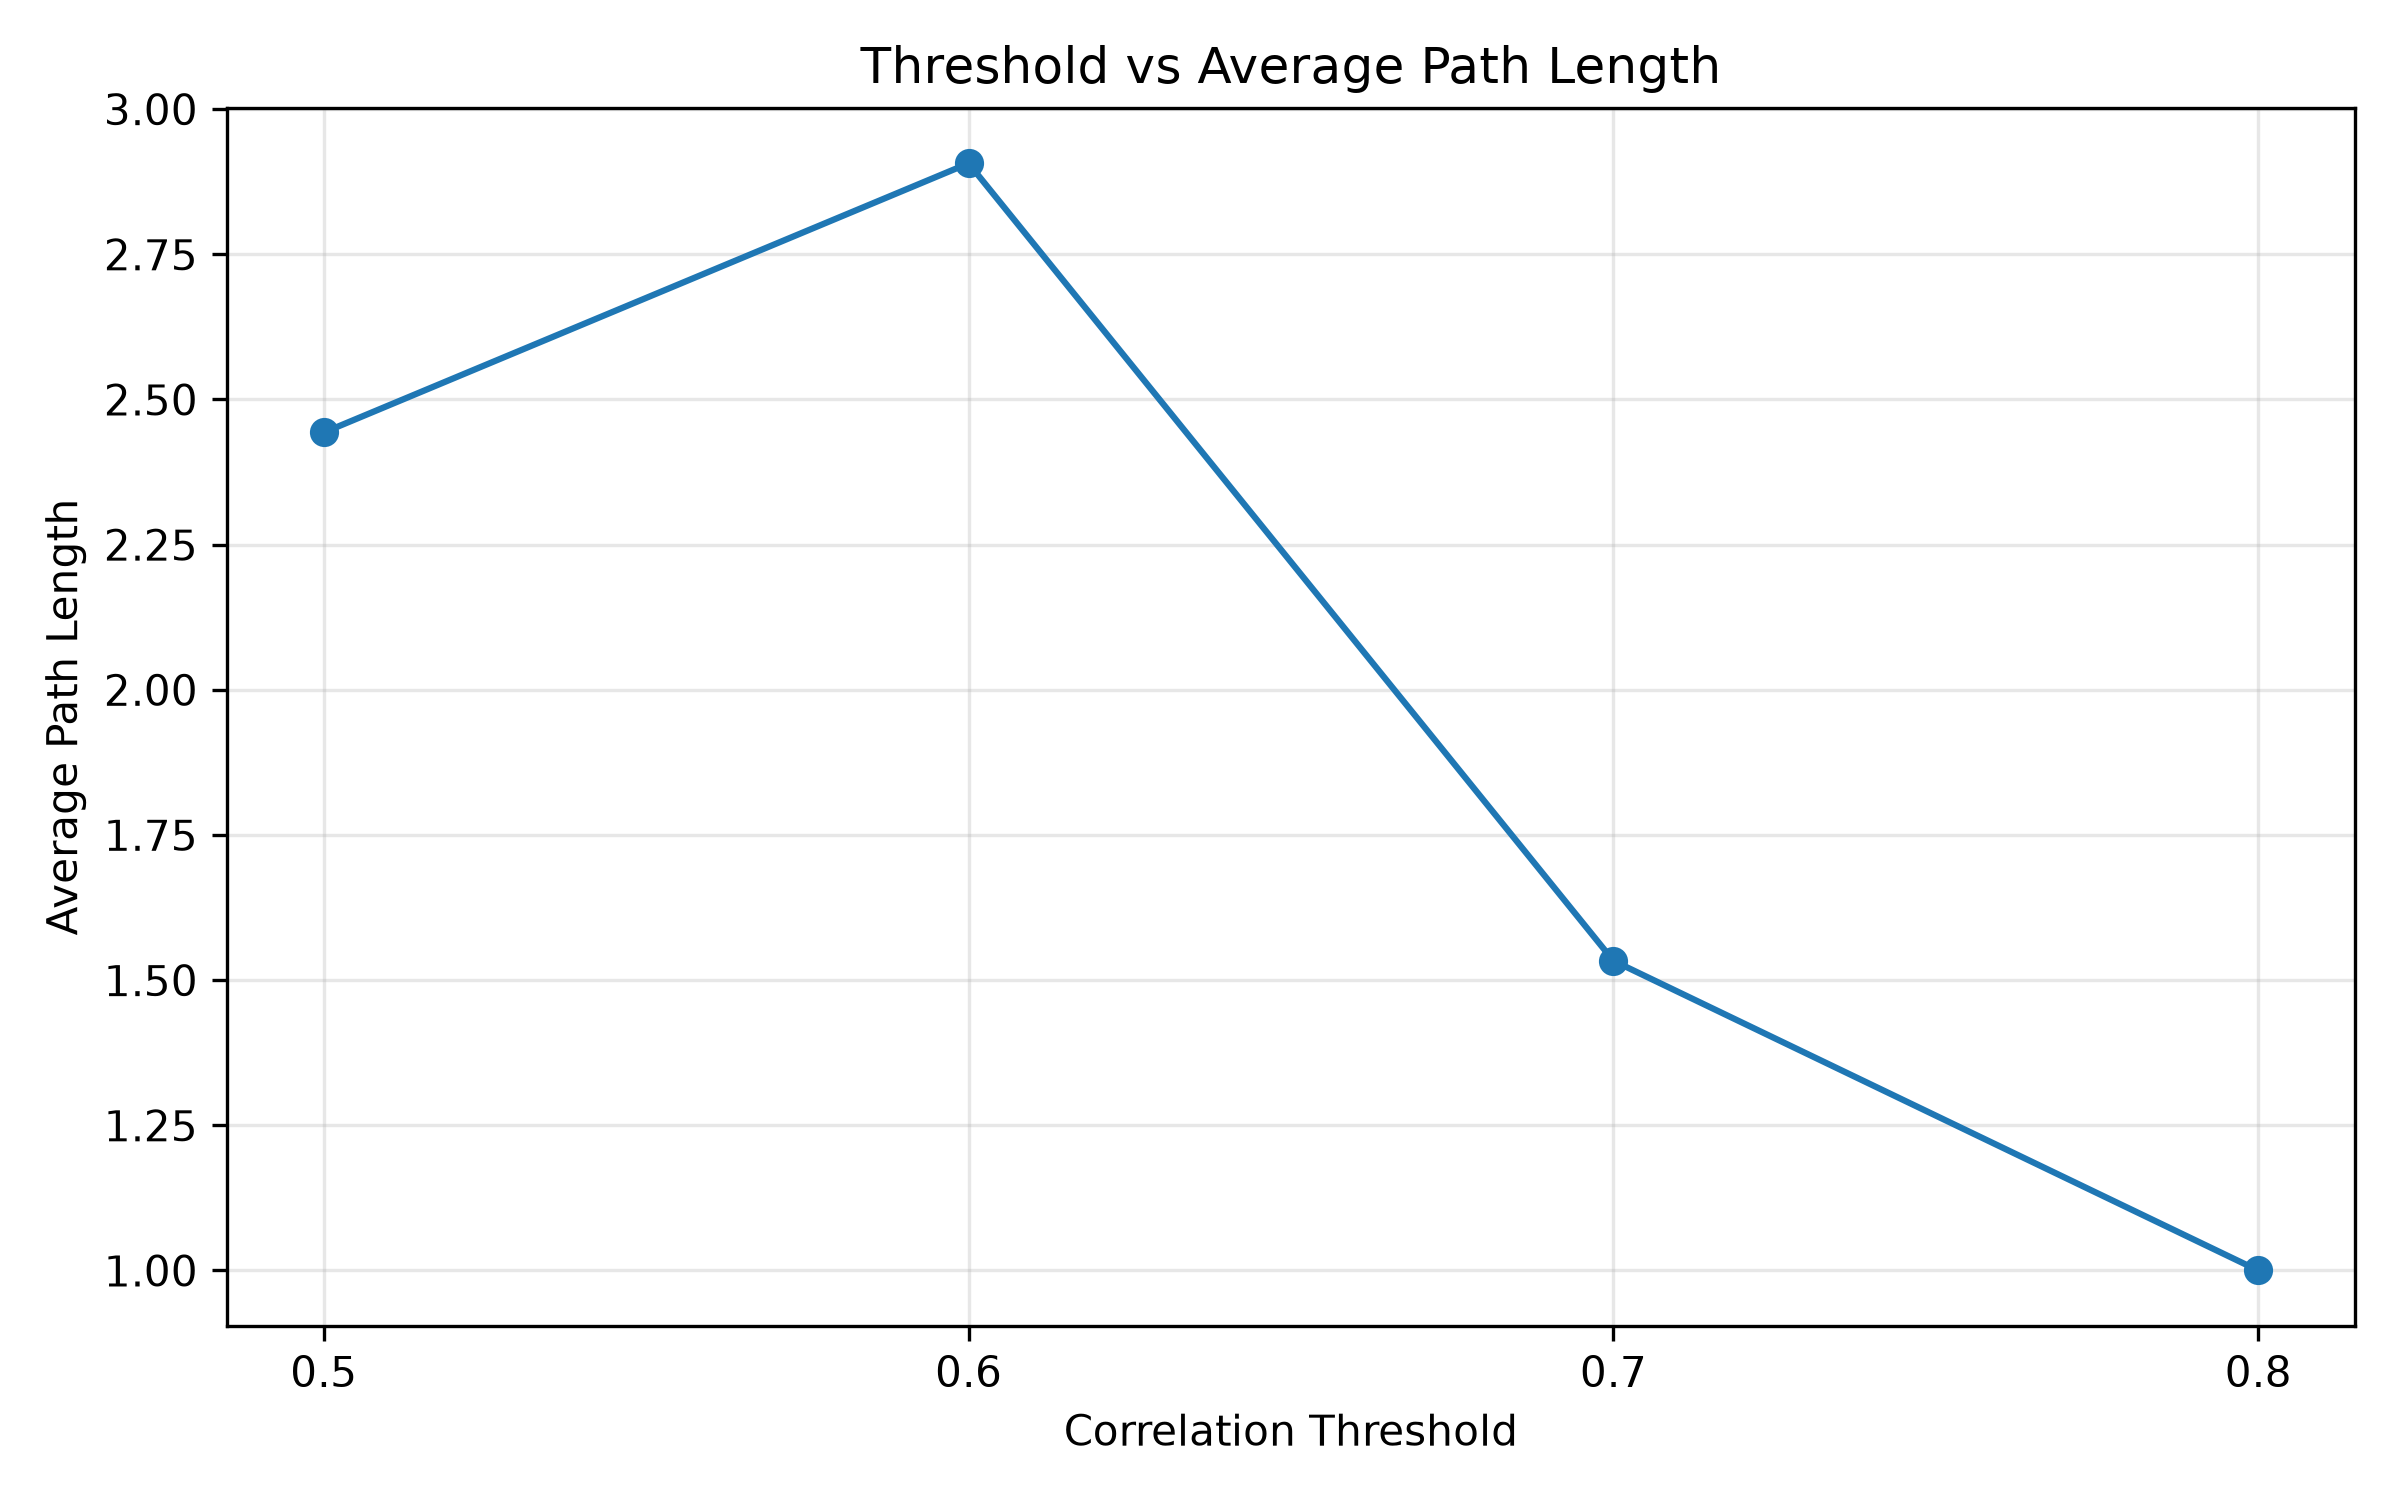
\includegraphics[width=0.85\textwidth]
    {threshold_vs_average_path_length.png}
    \caption{Effect of Correlation Threshold on Average Path Length}
    \label{fig:threshold_path}
\end{figure}

The average path length increases from approximately
2.44 at threshold 0.5 to 2.91 at threshold 0.6.

It then decreases to approximately 1.53 at threshold
0.7 and 1.00 at threshold 0.8.

The decrease at higher thresholds should be interpreted
carefully. At these thresholds, the largest connected
component becomes extremely small. Therefore, its
average path length is calculated over fewer nodes.

A lower average path length at a high threshold does
not mean that the overall network has become more
connected.

\subsection{Threshold Sensitivity Summary}

The results obtained from the generated sensitivity
plots are summarised below. Values are approximate
readings from the plotted results and should be
checked against the exact CSV output.

\begin{table}[H]
\centering
\caption{Network Structure at Different Correlation Thresholds}
\label{tab:threshold_summary}
\begin{tabular}{cccc}
\toprule
\textbf{Threshold} &
\textbf{Edges} &
\textbf{Giant Component} &
\textbf{Average Path Length}\\
\midrule
0.5 & 528 & 85 & 2.44\\
0.6 & 126 & 25 & 2.91\\
0.7 & 32 & 6 & 1.53\\
0.8 & 7 & 3 & 1.00\\
\bottomrule
\end{tabular}
\end{table}

The sensitivity analysis shows that the correlation
threshold has a major influence on network connectivity.

At lower thresholds, more companies are connected,
creating larger components.

At higher thresholds, only strongly correlated pairs
remain connected, resulting in a fragmented network.

The results also demonstrate why the choice of
threshold must be considered carefully when analysing
correlation-based financial networks.

% =================================================
\section{Interpretation and Discussion}
% =================================================

The analysis provides several insights into the
structural properties of the Indian stock market
network.

\subsection{Sparse Network Structure}

At the main threshold of 0.6, the network contains
184 nodes and 126 edges.

Its density is approximately 0.0075, indicating
that only a small fraction of all possible company
pairs are connected.

This suggests that strong positive return
relationships are concentrated among selected
company pairs.

\subsection{Fragmentation of the Network}

The network contains 122 connected components,
and its largest component consists of 25 companies.

A large number of companies remain isolated or
belong to small connected groups.

This indicates that the strongest return relationships
do not form one large connected structure across
the entire set of companies.

\subsection{Importance of Financial Services Companies}

Financial Services companies appear frequently
among the highest-ranked nodes in degree and
eigenvector centrality.

CANBK, PNB, BANKBARODA, BANKINDIA and UNIONBANK
are among the important companies according to
these measures.

This suggests that several financial companies
occupy structurally important positions in the
constructed network.

\subsection{Sector-Based Relationships}

The same-sector edge percentage is 81.75\%,
while sector assortativity is 0.7774.

Both results indicate that companies belonging
to the same industry sector tend to be connected
to one another.

Industry-related factors may contribute to
similar return movements among companies operating
in the same sector.

\subsection{Clustering}

The average clustering coefficient is 0.1962.

This indicates a modest degree of local clustering.
Some companies form groups in which their neighbours
are also connected to one another.

However, the network does not exhibit uniformly
high clustering across all companies.

\subsection{Threshold Dependence}

The sensitivity analysis demonstrates that network
structure changes substantially with the selected
correlation threshold.

At lower thresholds, the network has more edges
and larger connected components.

At higher thresholds, the network becomes more
fragmented because only stronger relationships
are retained.

Therefore, conclusions about network connectivity
should always be interpreted in relation to the
threshold used.

% =================================================
\section{Limitations of the Study}
% =================================================

Although the project provides useful insights into
the structure of the Indian stock market, it has
several limitations.

\subsection{Historical Constituents}

The study uses the current Nifty 200 constituent
list retrospectively for the entire study period.

Historical index membership was not incorporated.
As a result, the analysis may be affected by
survivorship or selection bias.

\subsection{Data Source Limitations}

Historical price information was obtained from
Yahoo Finance. Data availability and corporate-action
adjustments may differ across data providers.

The downloaded price series were checked for
unusual observations, but the accuracy of every
historical adjustment cannot be independently
guaranteed.

\subsection{Extreme Return Cleaning}

Selected extreme observations and dates were removed
during the cleaning process.

Although this helped maintain a common observation
panel, some removed movements may represent genuine
market information or corporate events.

In particular, the reason for every extreme observation
could not be conclusively verified.

\subsection{Pearson Correlation}

Pearson correlation measures linear relationships.
It may not capture nonlinear dependence between
stock returns.

Other methods, such as rank correlation or
alternative dependence measures, could be explored
in future research.

\subsection{Threshold Selection}

The network structure depends on the chosen
correlation threshold.

Different thresholds produce different numbers
of edges, connected components and centrality
rankings.

\subsection{Static Network}

The project constructs a network using one
combined study period.

Stock market relationships can change over time.
A static network cannot fully capture these
changes.

% =================================================
\section{Future Scope}
% =================================================

The project can be extended in several ways:

\begin{enumerate}
    \item \textbf{Dynamic Network Analysis:}
    Construct networks using rolling time windows
    to examine how company relationships change
    over time.

    \item \textbf{Weighted Networks:}
    Instead of converting correlations into binary
    edges, retain correlation values as edge weights.

    \item \textbf{Alternative Correlation Measures:}
    Use Spearman correlation or other dependence
    measures to capture different types of relationships.

    \item \textbf{Community Detection:}
    Apply community detection algorithms to identify
    groups of strongly connected companies.

    \item \textbf{Historical Index Constituents:}
    Use historical Nifty 200 membership to reduce
    survivorship-related limitations.

    \item \textbf{Sector Comparison:}
    Compare connectivity and centrality patterns
    across different industry sectors.

    \item \textbf{Financial Risk Analysis:}
    Study how market shocks may spread through
    connected companies and sectors.
\end{enumerate}

% =================================================
\section{Conclusion}
% =================================================

This project applied Network Science techniques
to analyse the topological and structural
relationships among companies in the Indian
stock market.

Historical adjusted closing prices were collected
for 200 Nifty 200 companies. After data verification,
preprocessing, return calculation and extreme
observation inspection, the final analysis used
184 companies and 735 common daily return observations.

Daily logarithmic returns were calculated and
Pearson correlation coefficients were obtained
between all pairs of companies.

An undirected, unweighted correlation network
was constructed using a main threshold of 0.6.
The resulting network contained 184 nodes and
126 edges, with a density of approximately 0.0075.

The network was found to be sparse and fragmented.
Its largest connected component contained
25 companies, while the network had 122 connected
components.

Centrality analysis identified CANBK and RECLTD
as important companies under different structural
measures. The average clustering coefficient
was 0.1962, indicating modest local clustering.

Sector analysis showed that approximately
81.75\% of the network edges connected companies
belonging to the same industry sector. The positive
assortativity coefficient of 0.7774 indicated
strong sector-based homophily.

Finally, threshold sensitivity analysis showed
that increasing the correlation threshold reduces
the number of edges and the size of the largest
connected component.

Overall, the study demonstrates that Network
Science provides a useful framework for understanding
relationships, connectivity patterns and structural
importance within the Indian stock market.

% =================================================
\section{References}
% =================================================

\begin{enumerate}

    \item Chi, K. T., Tse, C. K., Liu, J., \& Lau, F. C. M.
    (2010). A network perspective of the stock market.
    \textit{Journal of Empirical Finance, 17}(4), 659--667.

    \item Moghadam, M. K., et al. (2019).
    Complex networks analysis in Iran stock market:
    The application of centrality.
    \textit{Physica A: Statistical Mechanics and its Applications,
    531}, 121800.

    \item NSE Indices.
    \href{https://www.niftyindices.com/}
    {Official Nifty Indices Website}.

    \item Yahoo Finance.
    \href{https://finance.yahoo.com/}
    {Historical Stock Market Data}.

    \item NetworkX Developers.
    \href{https://networkx.org/}
    {NetworkX Documentation}.

    \item Python Software Foundation.
    \href{https://www.python.org/}
    {Python Programming Language}.

\end{enumerate}

\end{document}
